\documentclass[12pt]{article}
\usepackage{amsmath, amssymb, amsthm, epsfig, enumerate, xcolor}

\theoremstyle{definition}
\newenvironment{Proof}{\noindent {\sc Proof.}}{$\Box$ \vspace{2 ex}}
\newenvironment{Solution}{\noindent {\sc Solution.}}{$\Box$ \vspace{2 ex}}
\newcommand{\meq}{{\color{orange}\; =\;}}

\oddsidemargin-1mm
\evensidemargin-0mm
\textwidth6.5in
\topmargin-15mm
\textheight8.75in
\footskip27pt

\begin{document}

\noindent \text{\textbf{ENAE 685, Spring 2025}} \hspace{1.3cm} \text{\textbf{HOMEWORK 4}} \hspace{1.3cm} \\
\text{\textbf{Marvyn Bailly, Xiaohan Zhu}
} 
\vspace{1cm} 

\noindent {\bf Quantities defined}\\
$M_\infty$: Free-stream Mach number \\
$\gamma$: Ratio of specific heats \\
$u_\infty$: Free-stream velocity in $x$-direction (non-dimensionalized to 1)\\
$\omega$: Relaxation factor
\vspace{1cm} 


\noindent {\bf Include a short description of the problem and the theory behind potential flow and small disturbance assumptions. (15 points)}\\
To simplify the problem, we assume that the flow is inviscid and no rotation occurs at the initial and boundary condition, so the flow is irrotational everywhere. Then the continuity equation can be expressed as full potential:
\begin{equation}
    (\rho \phi_x)_x + (\rho \phi_y)_y = 0
\end{equation}
Where $\rho(x,y)$ depends on how we simplify the Navier-Stocks equation and can cause nonlinearity. From our derivation, we can assume that the disturbance in velocity, pressure, and density remains small, then we can rewrite the continuity equation as:
\begin{equation}
    A \phi_{xx} + \phi_{yy} = 0
\end{equation}
Where:
\begin{equation}
    A = 1 - M_\infty^2 - M_\infty^2(\gamma + 1) \frac{\phi_x}{u_\infty}
\end{equation}
If we additional assume that the potential disturbance in x direction is very small, then we can linearize this  as:
\begin{equation}
    A = 1 - M_\infty^2
\end{equation}
But this project tests for transonic flow, we still use the nonlinear approximation.\\
\vspace{1cm}



\noindent {\bf Include a description of the change in operator for supersonic flow, i.e. relaxation factor. In a numerical algorithm section, include a short description of the residual term and the P-operator}\\
In previous subsonic case, we uniformly set the relaxation factor to be greater than 1 for faster convergence. But for the transonic case, we need to keep $\omega$ exact equal to 1 in the supersonic regions to avoid instabilities and artificial diffusion. Additionally, we need to use upwind biased difference scheme in x direction in the supersonic region in order to align with the domain of influence. Therefore, we need to switch-like parameter to turn on and off different difference operator in different regions. Then the residual becomes:
\begin{equation}
\begin{aligned}
    L \phi_{j,k} &= ((1-\mu) A)_{j,k} D^C_{xx}(\Delta x_{j-1/2},\Delta x_{j+1/2}) \phi_{j,k} \\ 
    &+ (\mu A)_{j-1,k}D^B_{xx}(\Delta x_{j-3/2},\Delta x_{j-1/2}) \phi_{j-1,k} \\
    &+ D^C_{yy}(\Delta y_{k-1/2},\Delta y_{k+1/2}) \phi_{j,k}
\end{aligned}
\end{equation}
Where:
\begin{equation}
    \mu_{j,k} = \begin{cases}
        0, & \text{$A_{j,k}\geq 0$} \\
        1, & \text{$A_{j,k}< 0$} \\
    \end{cases}
\end{equation}
So that the $D^C_{xx}$ operator is turned on in the elliptic region, while the $D^B_{xx}$ operator is turned on in the hyperbolic region.\\
\\
The P-operator now also becomes:
\begin{equation}
    P_{ij} = (1-\mu) \left( \frac{\omega E_x^{-1}-2}{\Delta x^2(i-1,i,i+1)} + \frac{E_y^{-1}-2+E_y}{\Delta y^2} \right) + \mu \left( \frac{\omega E_x^{-2}-2E_x^{-1}+1}{\Delta x^2(i-2,i-1,i)} + \frac{E_y^{-1}-2+E_y}{\Delta y^2} \right)
\end{equation}
\vspace{1cm}


\noindent {\bf Briefly describe the computer implementation of the algorithm(s), as well as mention what type of computer was used. }\\
We used Python with NumPy to reimplement and modify the algorithm. Most parts of our code are identical to the subsonic version. All the major modifications are demonstrated below:\\
\\
In both the supersonic and subsonic case, a tri-diagonal system is solved because of the implicit treatment in y-direction, so the off-diagonal terms do not change. The diagonal term is changed because we are using upwind in x direction. That is, we modify the following code from:
\begin{verbatim}
b[k] = -(dym2[k] + dyp2[k] + A[j,k] * (dxm2[j] + dxp2[j]))
\end{verbatim}
To:
\begin{verbatim}
b[k] = -(1 - mu[j,k]) *(dym2[k] + dyp2[k] + A[j,k] * (dxm2[j] + dxp2[j])) \
        + mu[j-1,k] * A[j-1,k] * dxp2[j-1]
\end{verbatim}
Then we also change the RHS vector from:
\begin{verbatim}
f_arr[k] = -omega_jk[j,k] * (res[j, k] + A[j,k] * dphi[j-1, k] * dxm2[j])
\end{verbatim}
To
\begin{verbatim}
f_arr[k] = -omega_jk[j,k] * (1  - mu[j,k]) * \
        (res[j, k] + A[j,k] * dphi[j-1, k] * dxm2[j]) \
        + mu[j-1,k] * omega_jk[j,k] * A[j-1,k] * ((dxp2[j-1] + dxm2[j-1]) * \
        dphi[j-1, k] - dxm2[j-1] * dphi[j-2, k])
\end{verbatim}
Where \texttt{mu}, \texttt{omega\_jk} and \texttt{A} are defined beforehand as:
\begin{verbatim}
A = np.zeros((jmax, kmax))
for j in range(1, jmax-1):
    for k in range(1, kmax-1):
        A[j, k] = 1 - minf**2 - minf**2*(gamma + 1) * 1 * dx[j] * \
                ( (phi[j+1, k] - phi[j, k]) * (x[j] - x[j-1]) \
                / (x[j+1] - x[j]) + (phi[j, k] - phi[j-1, k]) \
                * (x[j+1] - x[j]) / (x[j] - x[j-1]))
mu = np.where(A >= 0, 0, 1)
omega_jk = np.ones((jmax, kmax)) * omega
omega_jk[A <= 0] = 1
\end{verbatim}
All computations were performed on a Dell XPS laptop.  


\vspace{1cm}


\noindent {\bf Attach a source listing of the program in an appendix at the end of the report.}\\
Please refer to the Appendix section of this document.\\

\vspace{1cm}


\noindent {\bf Attach a sample input and a sample output as additional appendices.}\\
Please refer to the Appendix section of this document to see a sample input and output of the code.\\

\vspace{1cm}

\noindent {\bf You may want to run one case with the same parameters as in your code from Problem Set \#3 and include in the report, to verify to me as well as yourself that you obtain the same results.}\\

To verify the correctness of the code, we compute a subsonic case to compare with the pre-existing MATLAB code. We compute the flow about a NACA 0010 airfoil (TH = 0.10) for $M_\infty = 0.0$ (incompressible) without wind tunnel wall (iwall = 0) and with a default grid of:

\begin{center}
\begin{tabular}{@{} l l l l @{}}
    JLE = 33  & JTE = 63  & JMAX = 95  & KMAX = 33 \\
    DXDY = 1  & XSF = 1.18  & YSF = 1.18  & KCONST = 3
\end{tabular}    
\end{center}

Plotting the pressure distribution along the airfoil surface, we obtain the plot shown in Figure \ref{fig:pressure_coefficient-1}. For comparison, the same plot is shown in Figure \ref{fig:pressure_coefficient-1} generated from the MATLAB code.  We can see from the plots, that the pressure distribution is the same and the number of iterations required to reduce the $L_2$ norm of the residual by approximately three orders of magnitude is also the same. Furthermore, we can see that the pressure distribution in both cases follows the Prandtl-Glauert correction to data from Abbot and von Doenhoff for linearized compressible flow. This shows that the Python code is working correctly.

% \begin{figure}
%     \centering
%     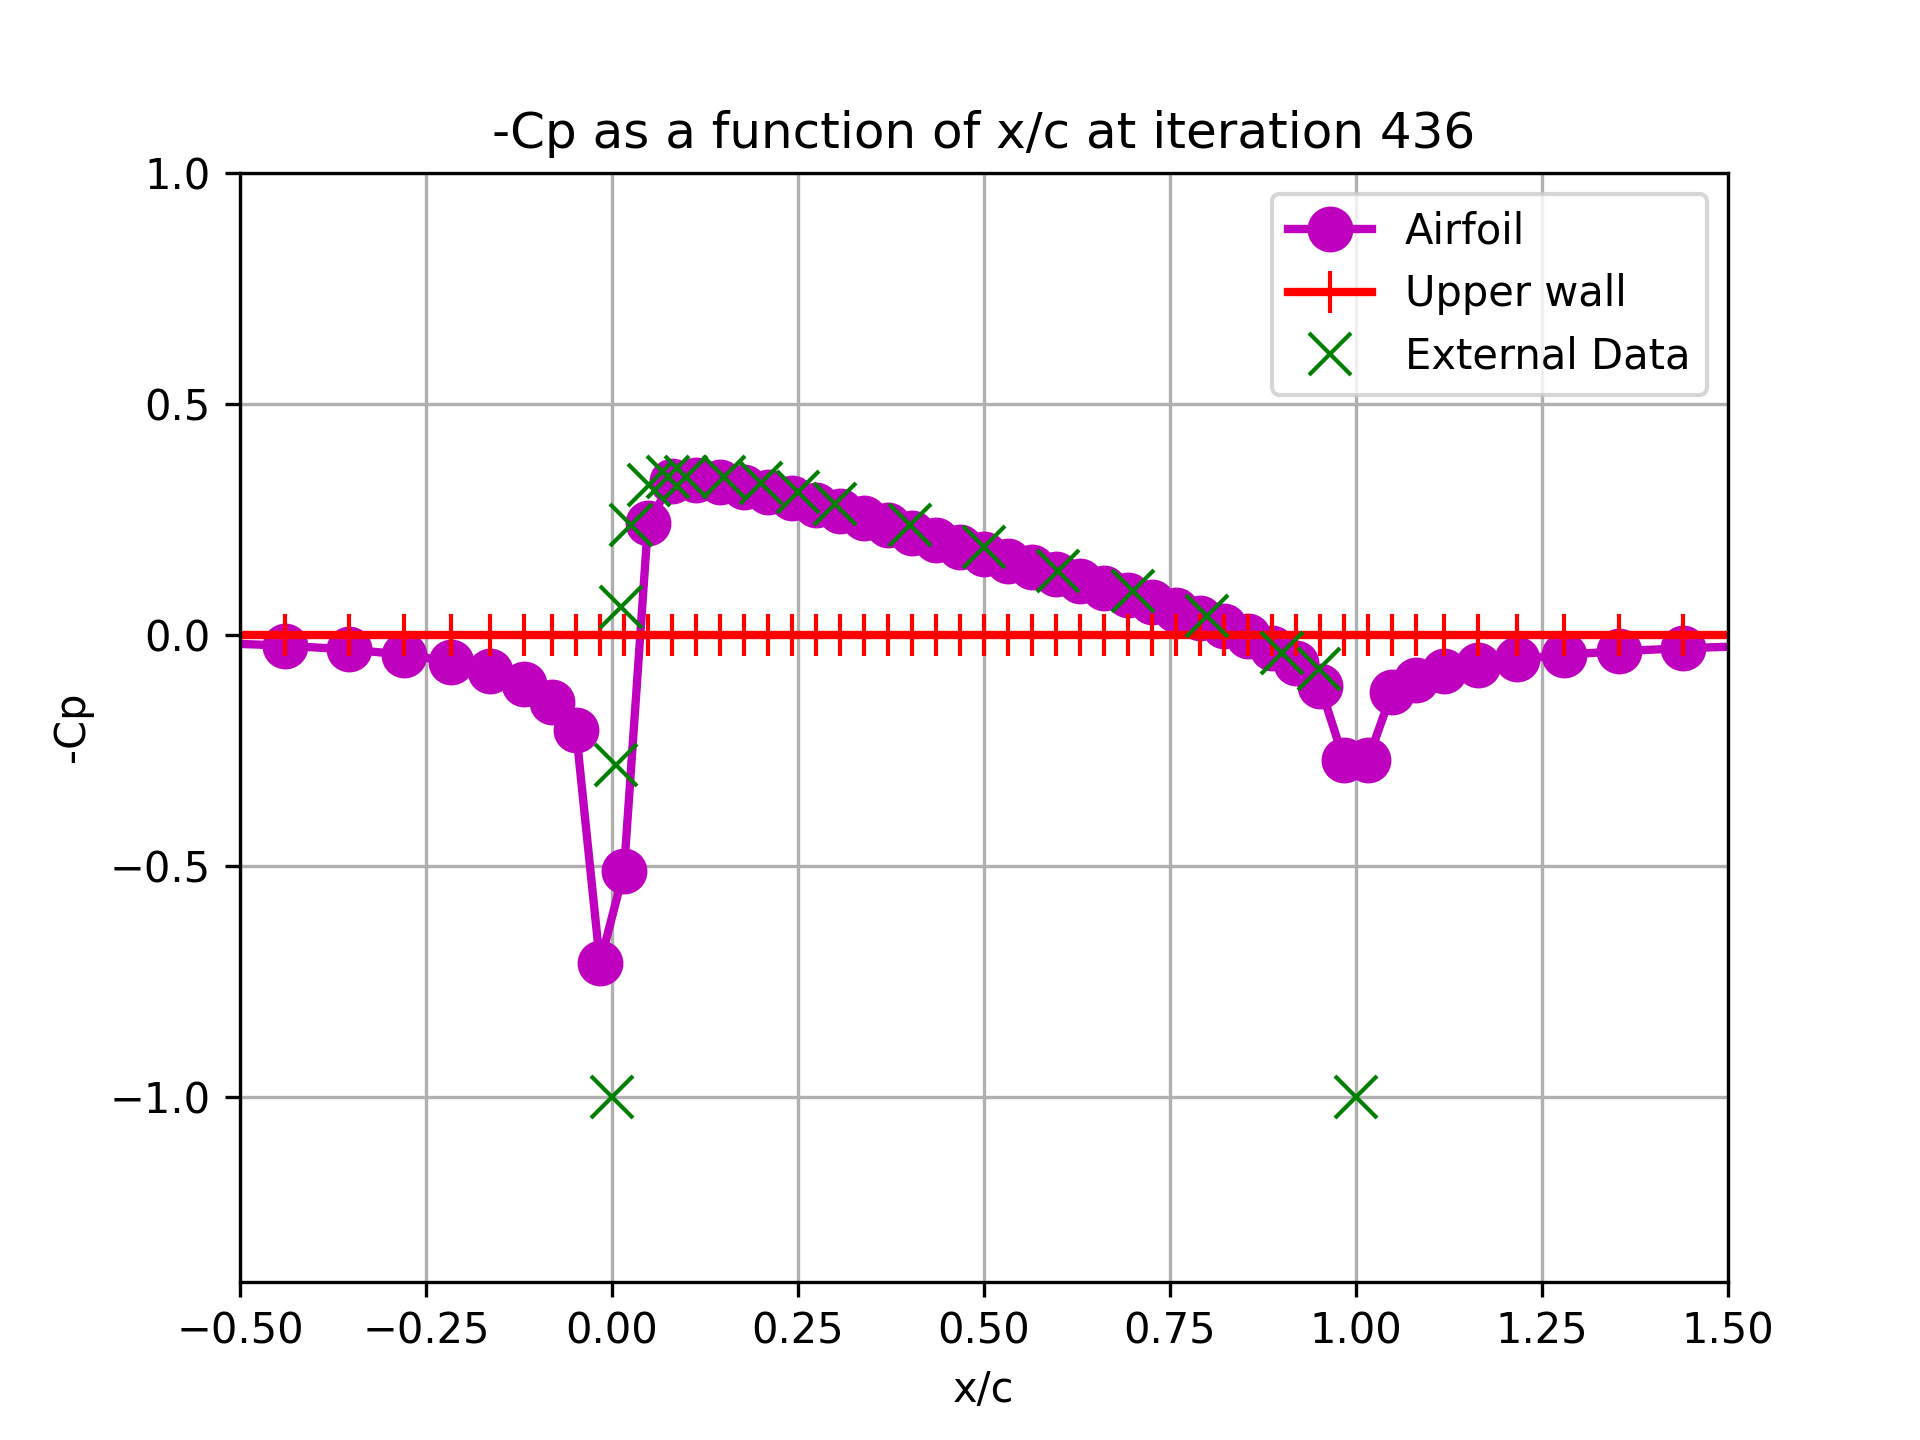
\includegraphics[width=0.75\textwidth,height=\textwidth,keepaspectratio]{images/pressure_coefficient-1.png}
%     \caption{Pressure distribution along the airfoil surface for NACA 0010 airfoil at $M_\infty = 0.0$ using Python code.}
%     \label{fig:pressure_coefficient-1}
% \end{figure}

% \begin{figure}
%     \centering
%     \includegraphics[width=0.75\textwidth,height=\textwidth,keepaspectratio]{images/pressure_coefficient-0.png}
%     \caption{Pressure distribution along the airfoil surface for NACA 0010 airfoil at $M_\infty = 0.0$ using MATLAB code.}
%     \label{fig:pressure_coefficient-0}
% \end{figure}

\vspace{1cm}


\noindent {\bf Include a table showing the different cases run, the number of iterations required for convergence, number of supersonic points, total CPU time, etc.}\\

We continue to run the code for a NACA 0010 airfoil and a biconvex airfoil (TH = 0.10) for $M_\infty = 0.75$ and $M_\infty = 0.8$ in air ($\gamma = 1.4$) respectively. These computations are done with a default grid of

\begin{center}
    \begin{tabular}{@{} l l l l @{}}
        JLE = 33  & JTE = 73  & JMAX = 105  & KMAX = 43 \\
        DXDY = 1  & XSF = 1.2  & YSF = 1.2  & KCONST = 3
    \end{tabular}    
\end{center}


We also preform two additional cases, first a NACA 0010 airfoil at $M_\infty = 0.75$ with the wind tunnel one chord above the centerline (with equal spacing in the y-direction) and secondly a NACA 0010 airfoil at $M_\infty = 0.80$ using a fine grid of

\begin{center}
    \begin{tabular}{@{} l l l l @{}}
        JLE = 63  & JTE = 123  & JMAX = 185  & KMAX = 63 \\
        DXDY = 1  & XSF = 1.1  & YSF = 1.0  & KCONST = 3
    \end{tabular}    
\end{center}

All cases were run until either the number of iterations exceeded 1000 or the $L_2$ norm of the residual was reduced by three orders of magnitude. The number of iterations required, the number of supersonic points at the final iteration, and the total CPU time are summarized in Table \ref{tab:results}. From now on, we will refer to each set of parameters using the case number presented in \ref{tab:results}.

\begin{table}[h]
    \centering
    \begin{tabular}{c l c c c c c c}
        \hline
        Case & Airfoil & $M_\infty$ & Grid Type & Wind Tunnel & Iterations & Supersonic Points & CPU Time (s) \\
        \hline
        1 & NACA 0010 & 0.75 & Default & None & 1000 & 0 & 19.9 \\
        2 & Biconvex & 0.75 & Default & None & 601 & 0 & 12.1 \\
        3 & NACA 0010 & 0.80 & Default & None & 1000 & 10 & 20.1 \\
        4 & Biconvex & 0.80 & Default & None & 1000 & 21 & 19.9 \\
        5 & NACA 0010 & 0.75 & Default & Yes & 1000 & 1 & 20.19 \\
        6 & NACA 0010 & 0.80 & Stretched & None & 1000 & 18 & 52.9 \\
        \hline
    \end{tabular}
    \caption{Summary of computations: number of iterations, supersonic points, and CPU time.}
    \label{tab:results}
\end{table}

\vspace{1cm}



\noindent {\bf Include figures that show the pressure distribution on the airfoil by plotting the pressure coefficient versus x/c along the airfoil. Try to verify the pressure distribution by independent means.}\\

We can plot the pressure distribution on the airfoil $-C_p$ and compare it to $x/c$ along the airfoil. The results for cases 1-6 are shown in Figures \ref{fig:pressure_coefficient-2} - \ref{fig:pressure_coefficient-7} respectively. We note that the green points are Prandtl-Glauert correction to data from Abbot and von Doenhoff which mostly align with our NACA0010 cases, verifying that the solution is approximately accurate.

\begin{figure}
    \centering
    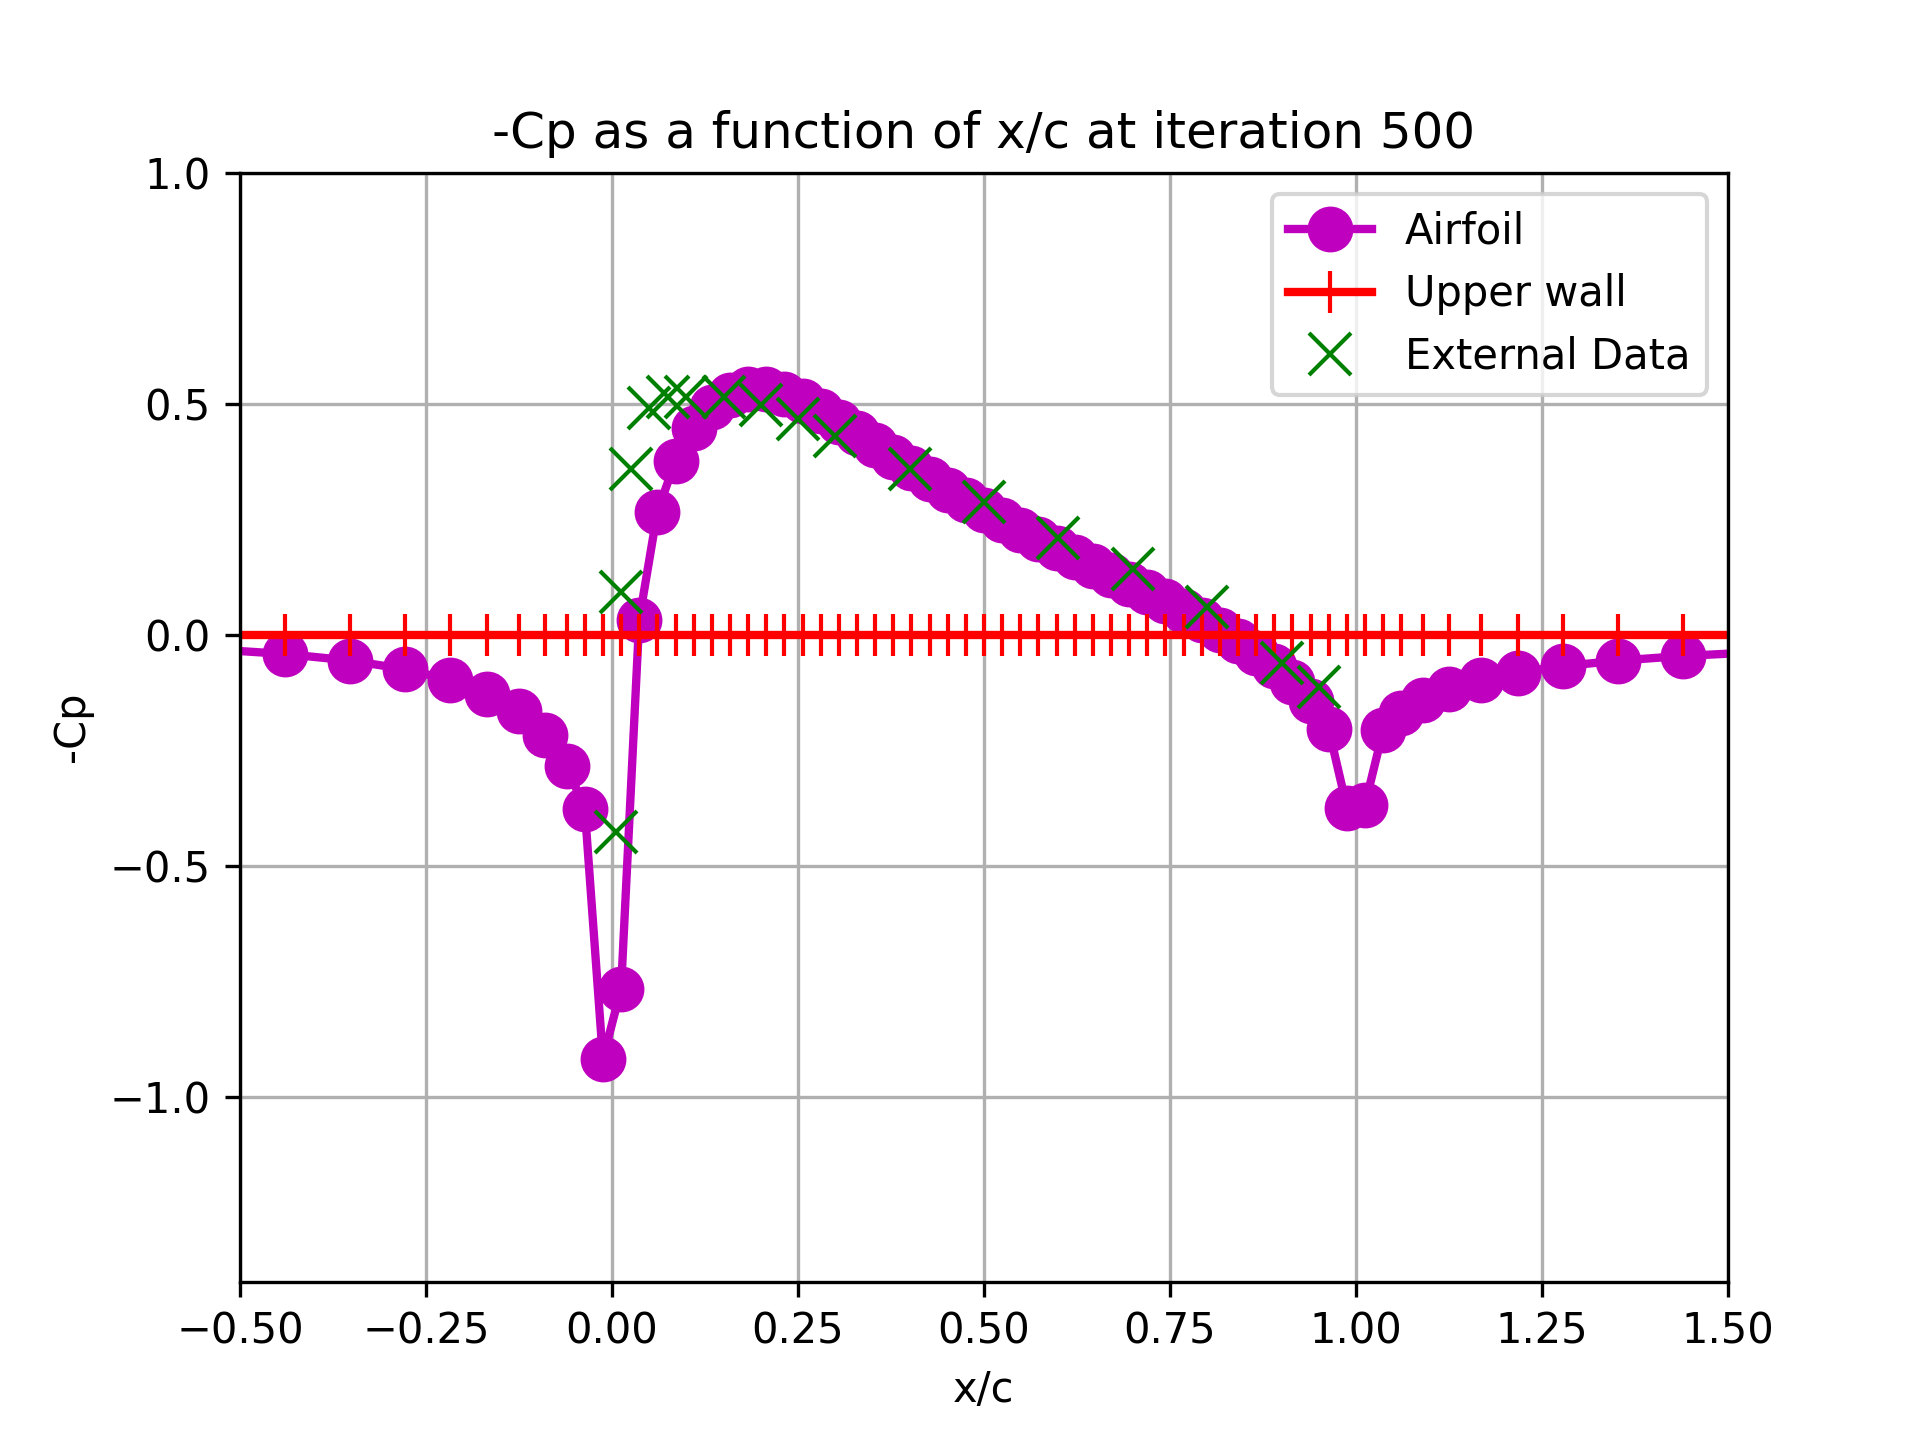
\includegraphics[width=0.75\textwidth,height=\textwidth,keepaspectratio]{images/pressure_coefficient-2.png}
    \caption{Pressure distribution $-C_p$ compared to $x/c$ along the airfoil surface for NACA 0010 airfoil at $M_\infty = 0.75$.}
    \label{fig:pressure_coefficient-2}
\end{figure}

\begin{figure}
    \centering
    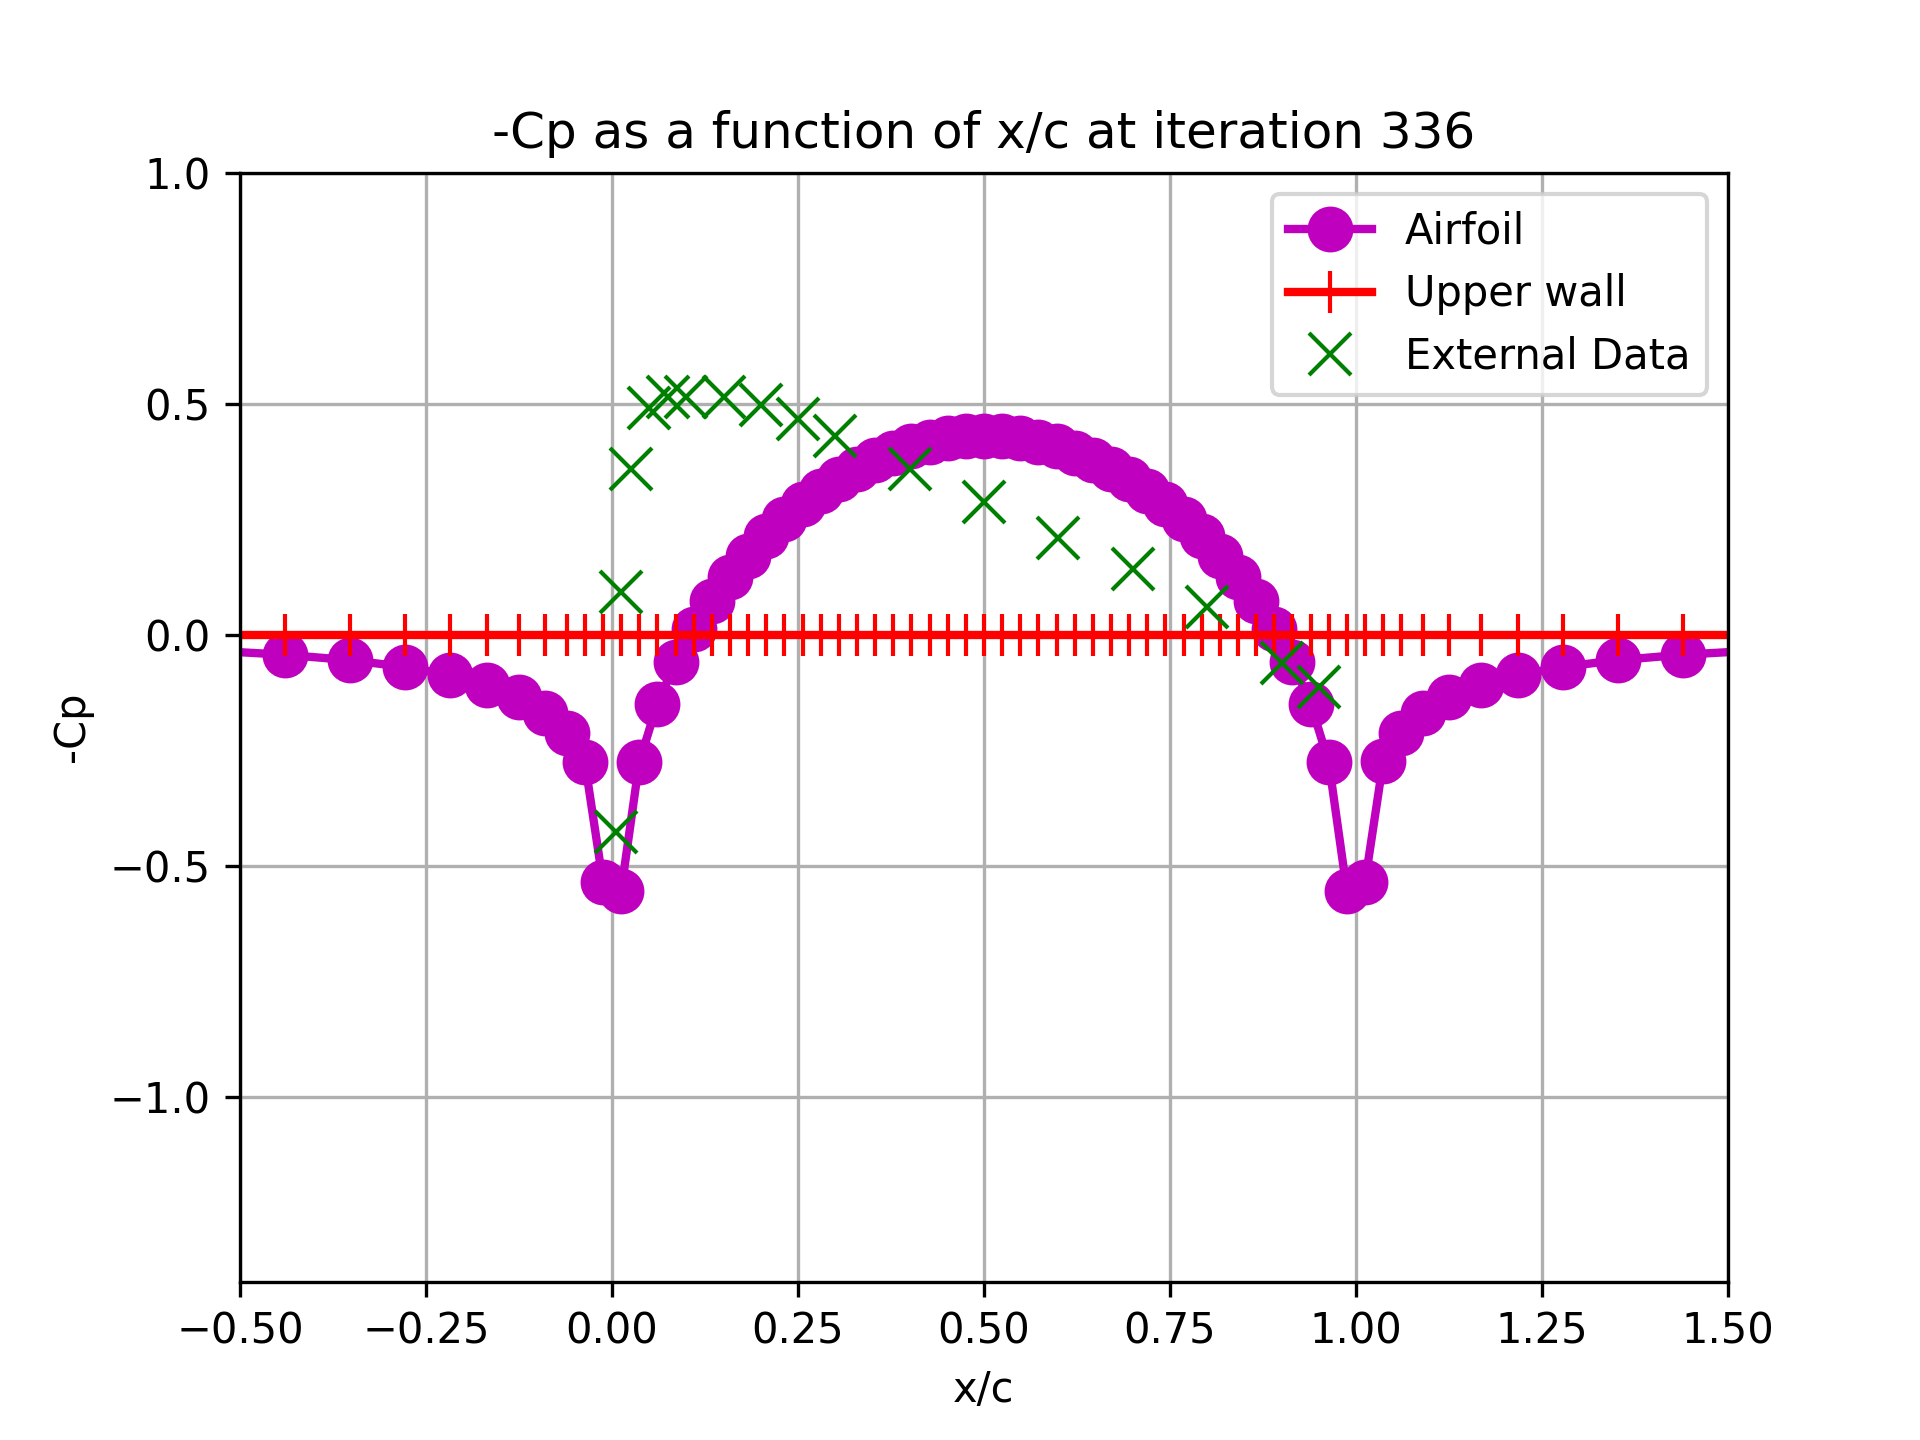
\includegraphics[width=0.75\textwidth,height=\textwidth,keepaspectratio]{images/pressure_coefficient-3.png}
    \caption{Pressure distribution $-C_p$ compared to $x/c$ along the airfoil surface for Biconvex 0010 airfoil at $M_\infty = 0.75$.}
    \label{fig:pressure_coefficient-3}
\end{figure}

\begin{figure}
    \centering
    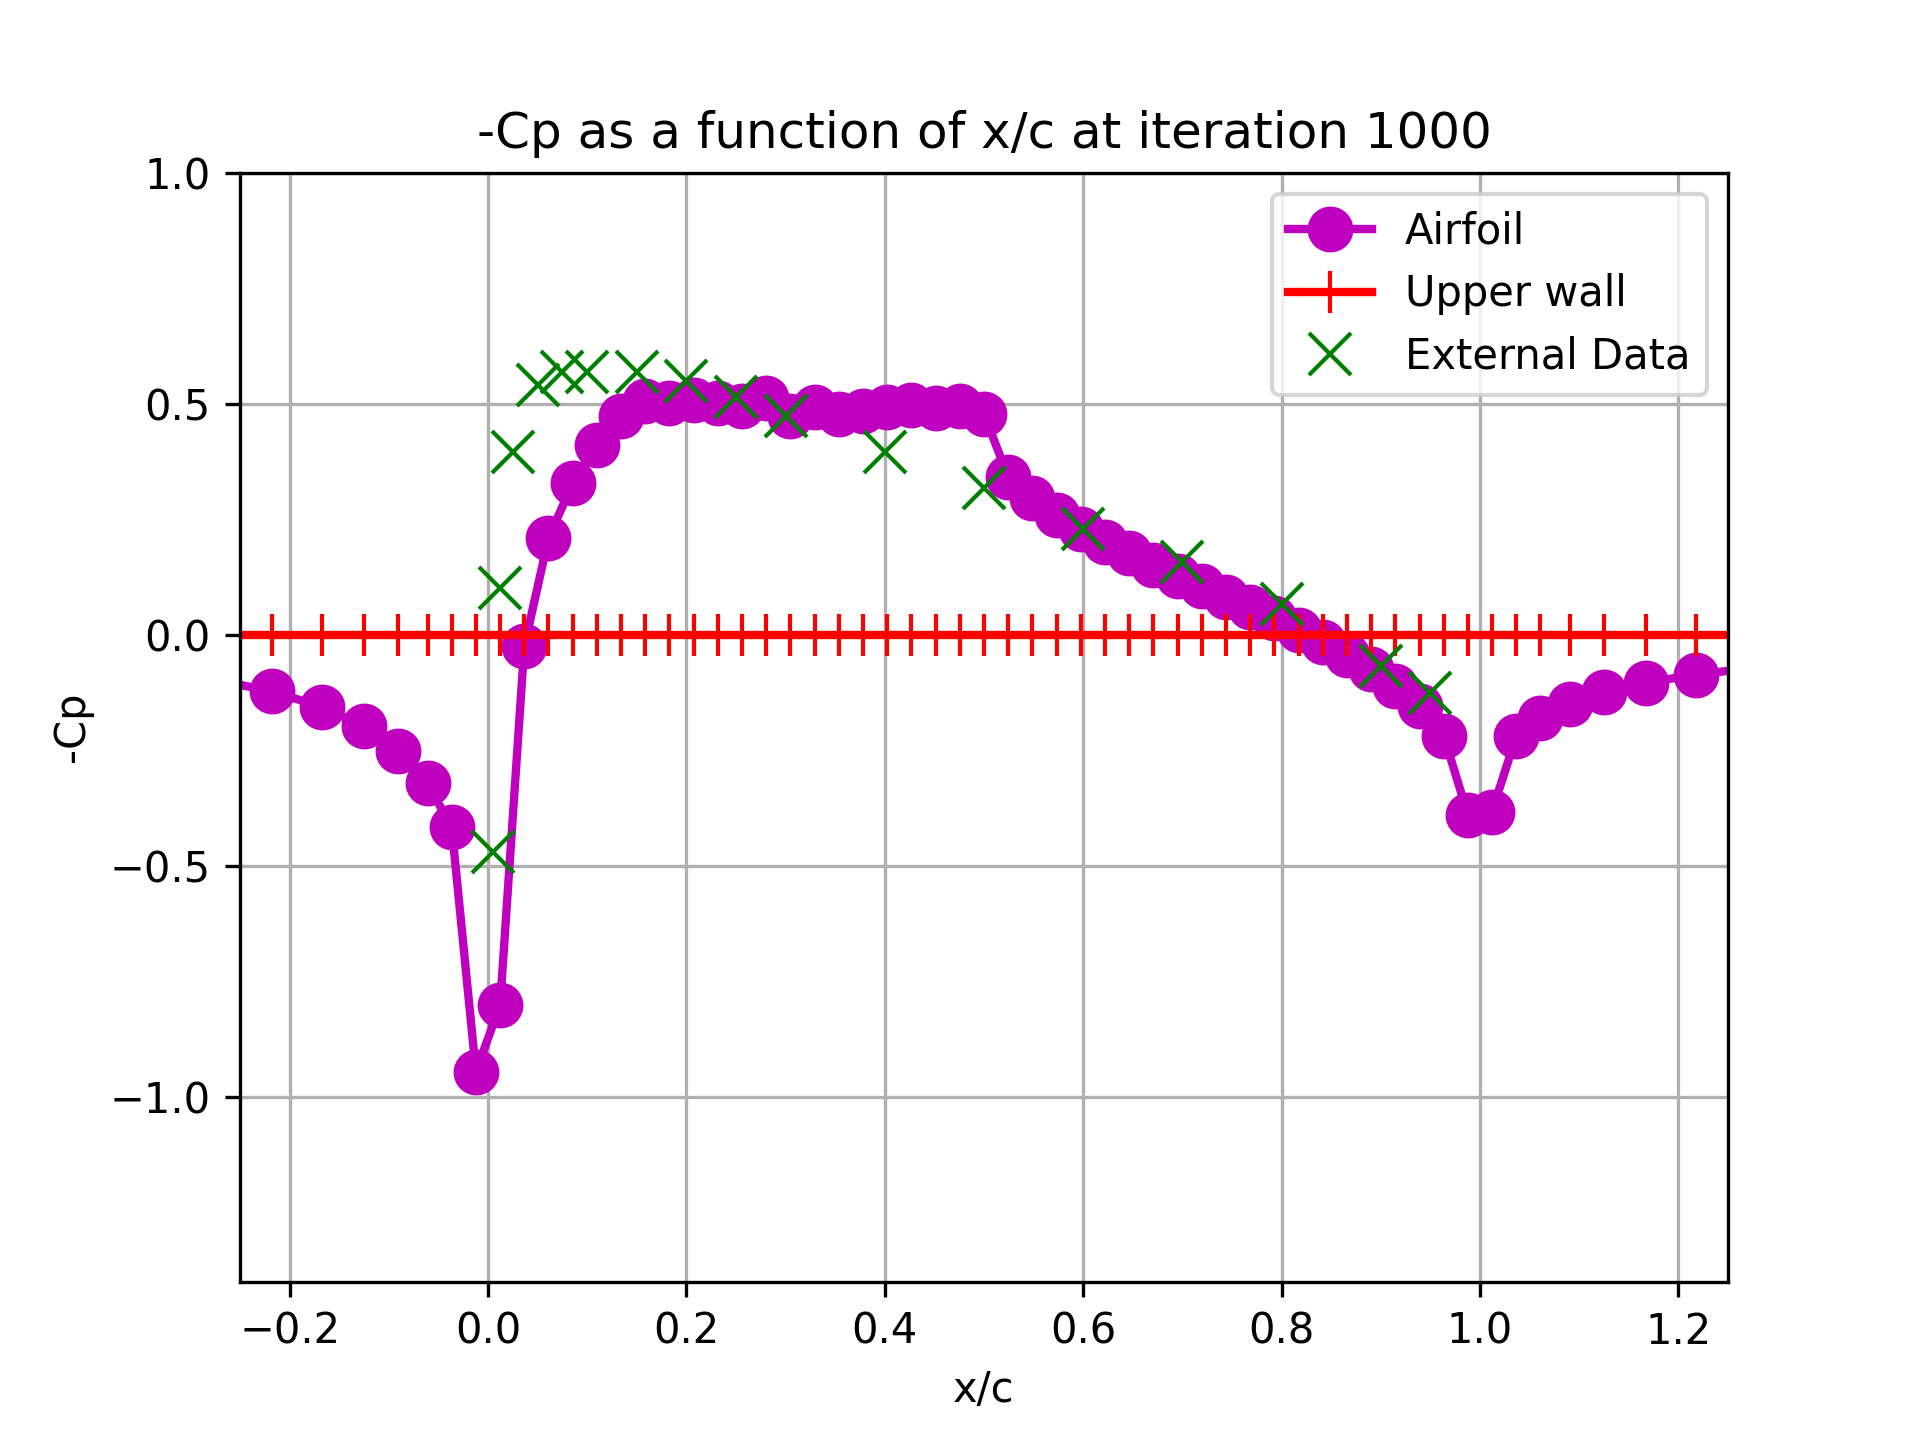
\includegraphics[width=0.75\textwidth,height=\textwidth,keepaspectratio]{images/pressure_coefficient-4.png}
    \caption{Pressure distribution $-C_p$ compared to $x/c$ along the airfoil surface for NACA 0010 airfoil at $M_\infty = 0.80$.}
    \label{fig:pressure_coefficient-4}
\end{figure}

\begin{figure}
    \centering
    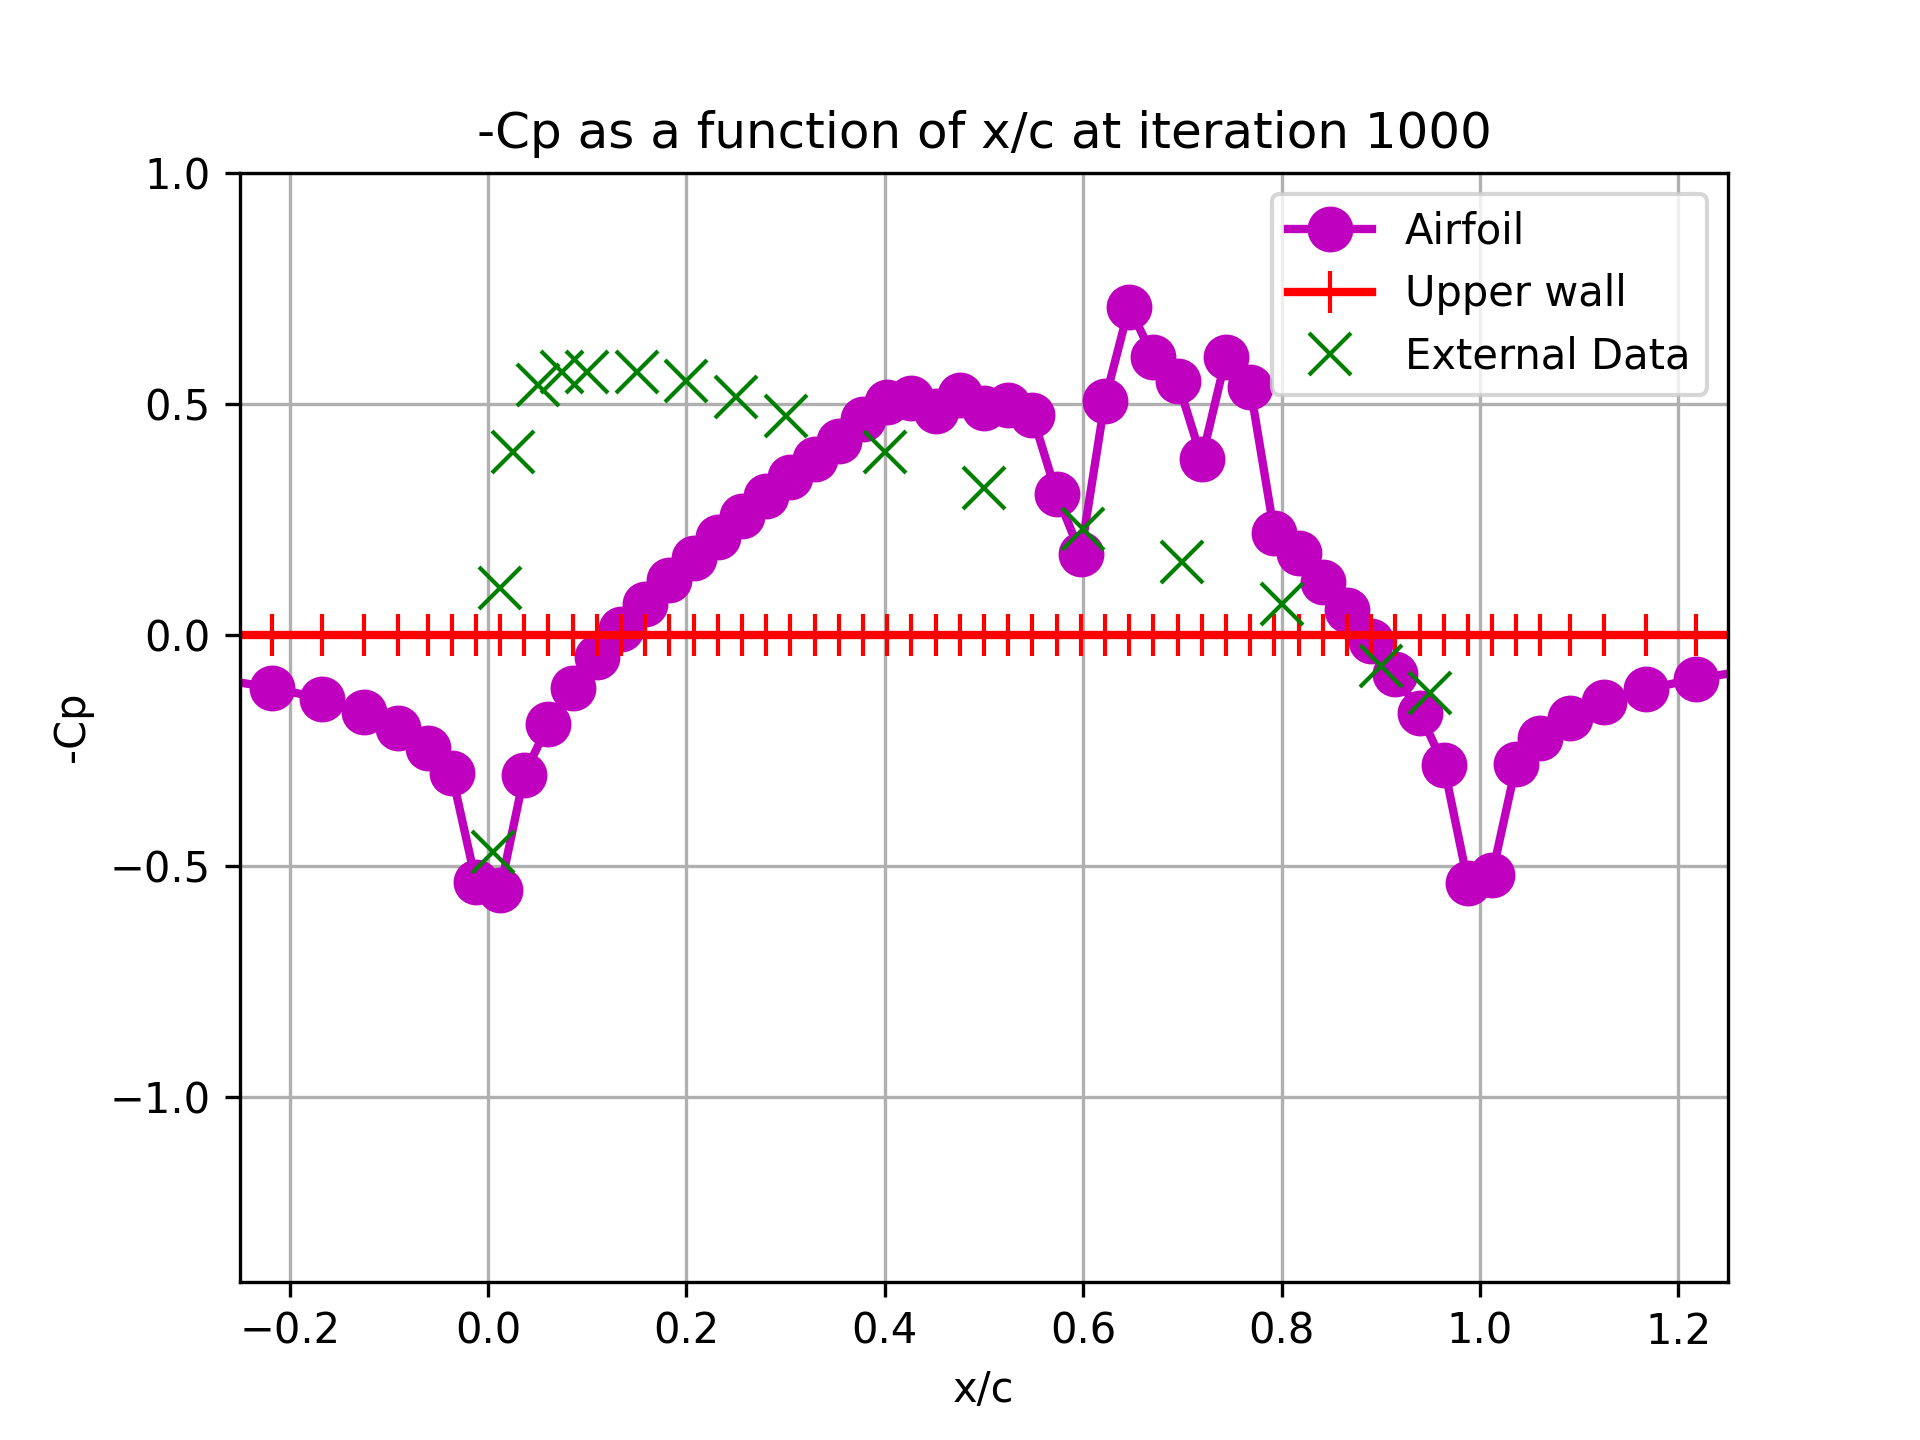
\includegraphics[width=0.75\textwidth,height=\textwidth,keepaspectratio]{images/pressure_coefficient-5.png}
    \caption{Pressure distribution $-C_p$ compared to $x/c$ along the airfoil surface for Biconvex 0010 airfoil at $M_\infty = 0.80$.}
    \label{fig:pressure_coefficient-5}
\end{figure}

\begin{figure}
    \centering
    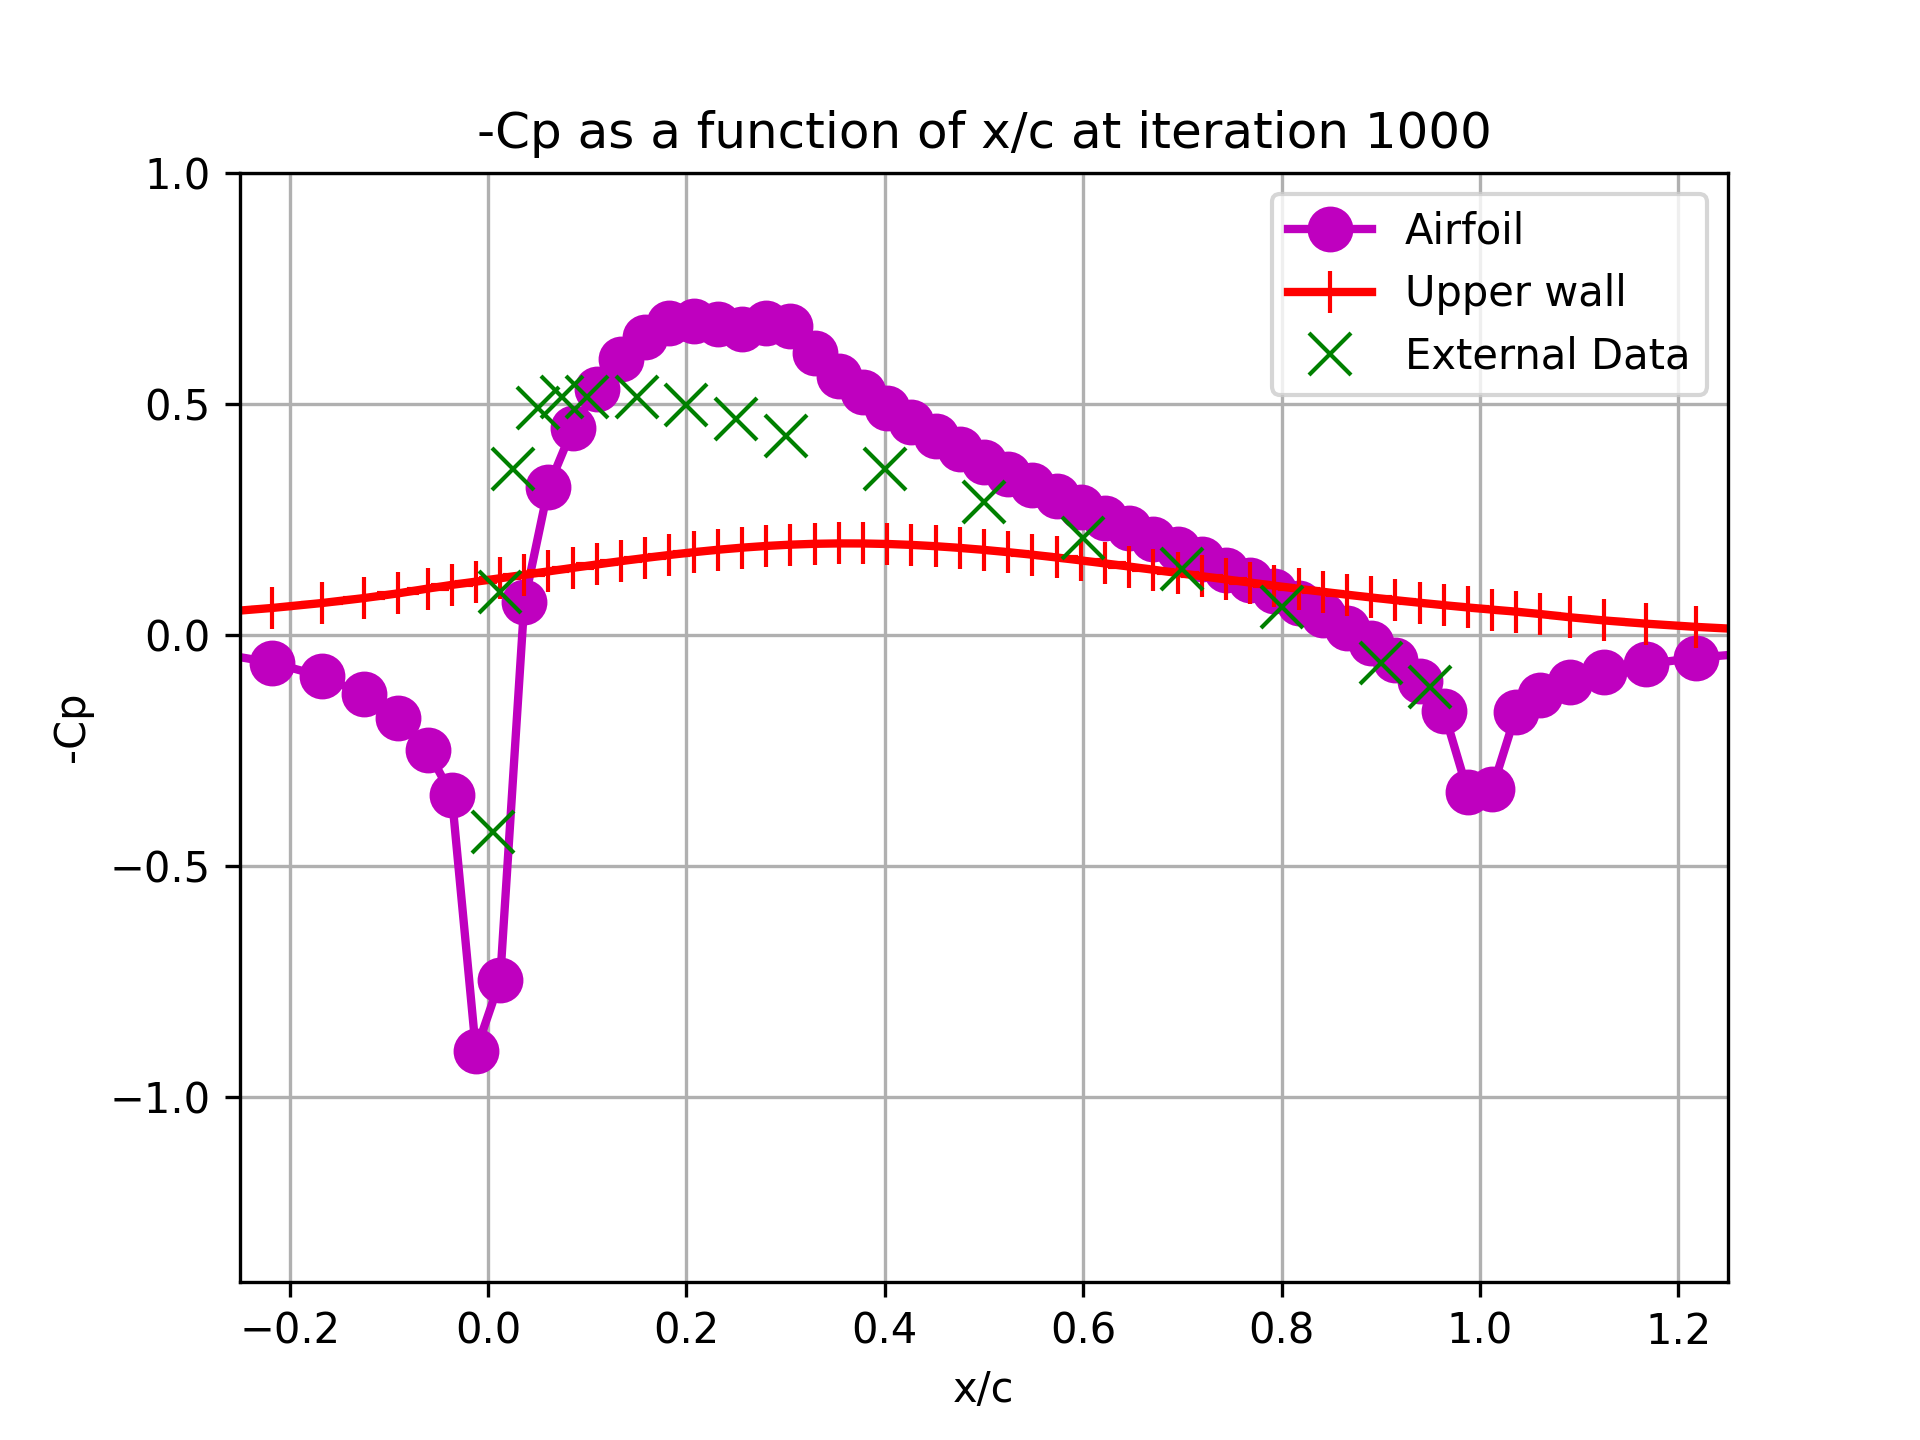
\includegraphics[width=0.75\textwidth,height=\textwidth,keepaspectratio]{images/pressure_coefficient-6.png}
    \caption{Pressure distribution $-C_p$ compared to $x/c$ along the airfoil surface for NACA 0010 airfoil at $M_\infty = 0.75$ with a wind tunnel.}
    \label{fig:pressure_coefficient-6}
\end{figure}

\begin{figure}
    \centering
    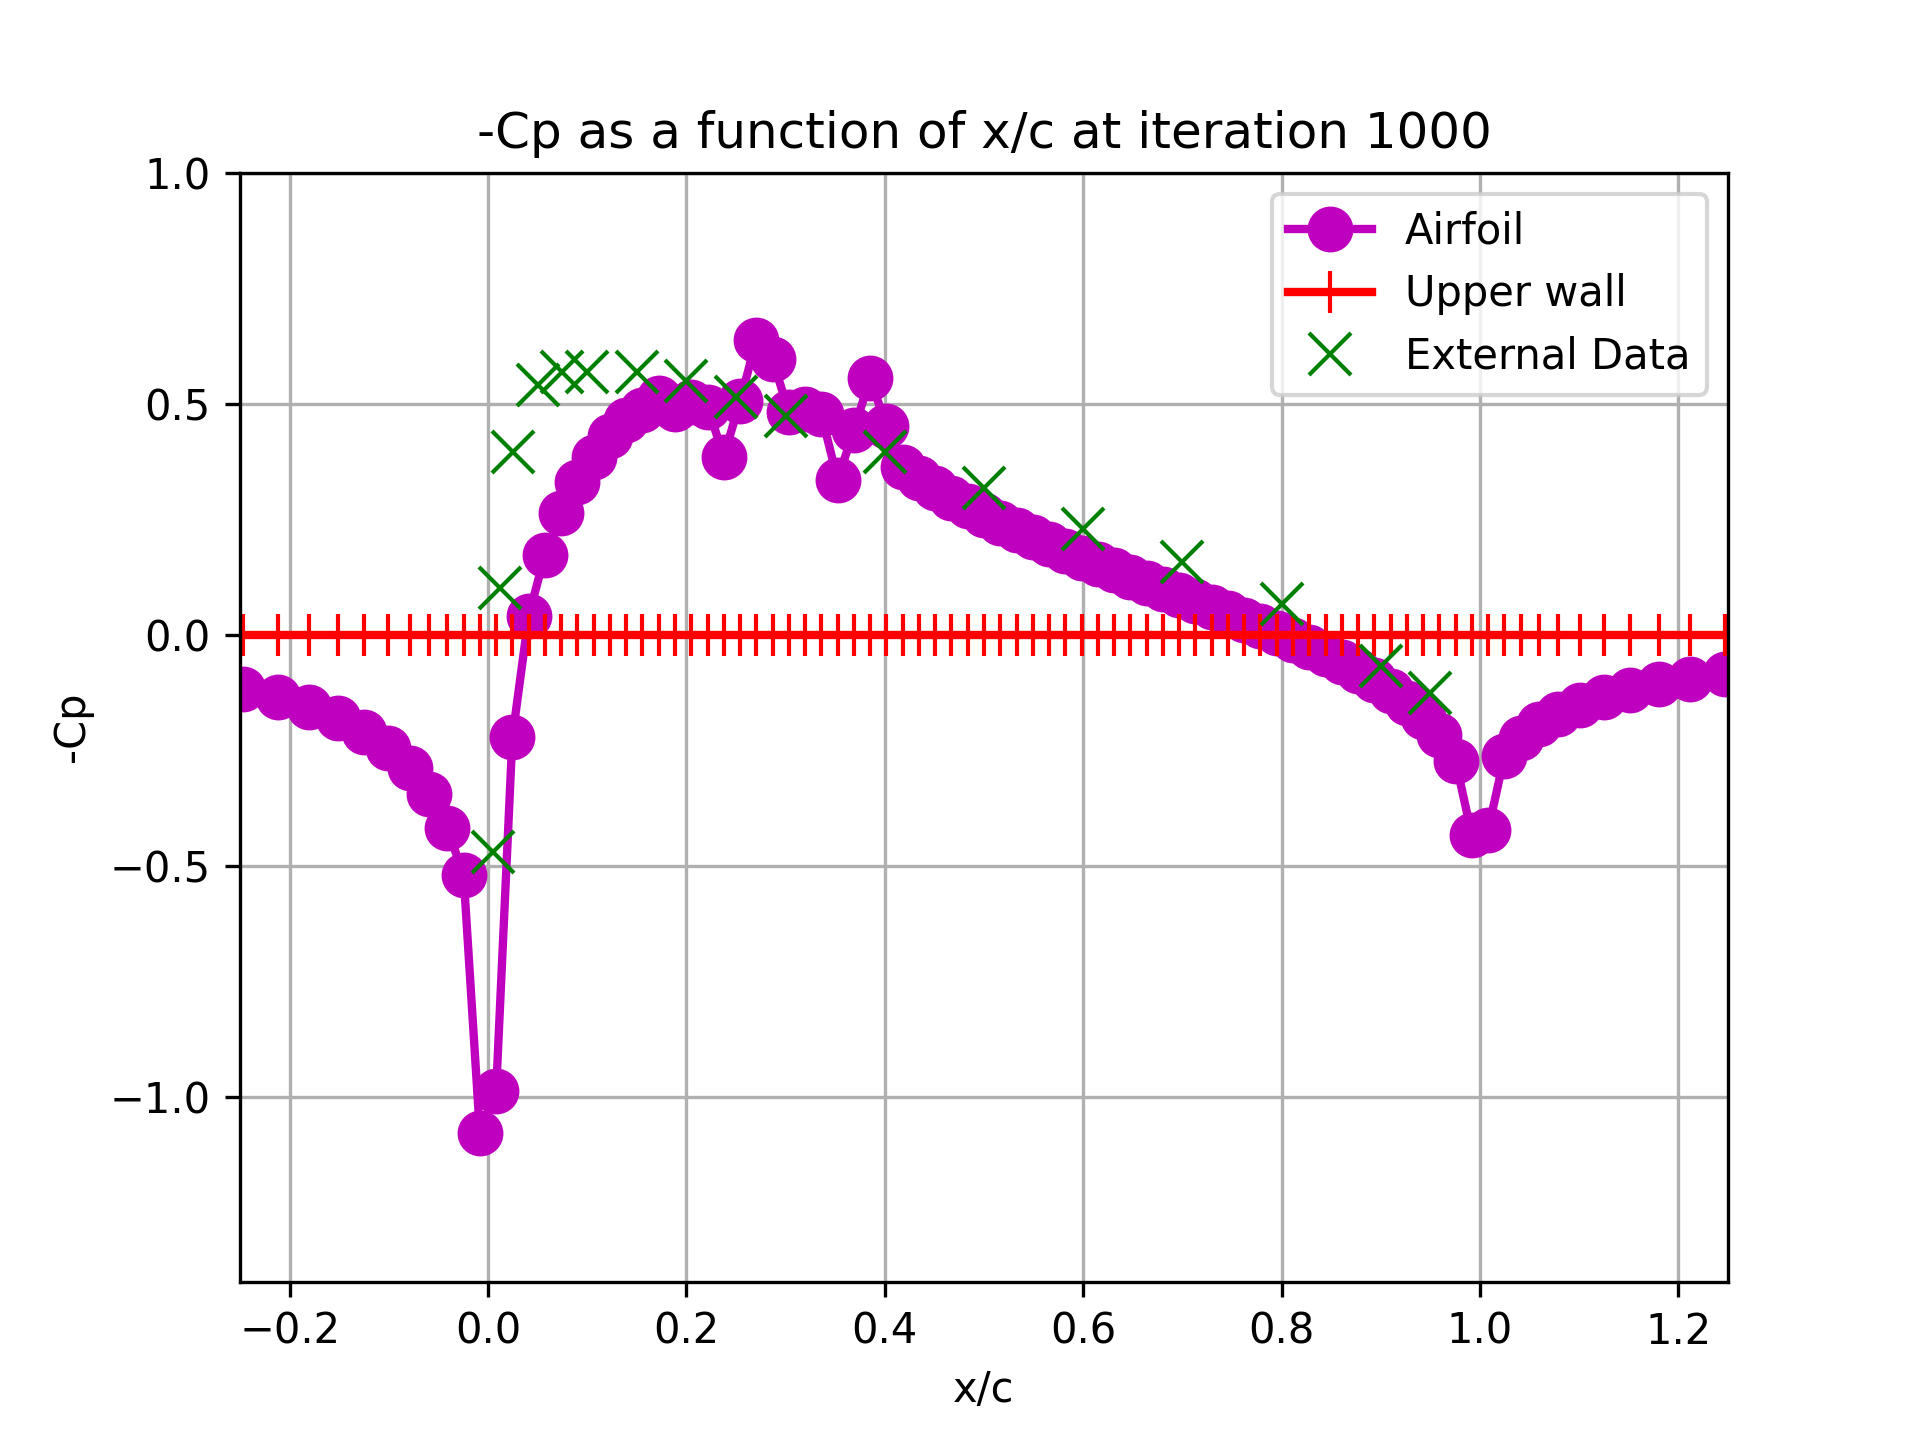
\includegraphics[width=0.75\textwidth,height=\textwidth,keepaspectratio]{images/pressure_coefficient-7.png}
    \caption{Pressure distribution $-C_p$ compared to $x/c$ along the airfoil surface for NACA 0010 airfoil at $M_\infty = 0.80$ using a stretched mesh.}
    \label{fig:pressure_coefficient-7}
\end{figure}

\vspace{1cm}


\noindent {\bf Plot the representative convergence histories showing the log10 of the L2 norm of the residual versus iteration number. }\\

We can plot the $log_{10}$ of the $L^2$ norm of the residual versus the iteration number for cases 1-6 as shown in Figure \ref{fig:residual_history-7.png}.

\begin{figure}
    \centering
    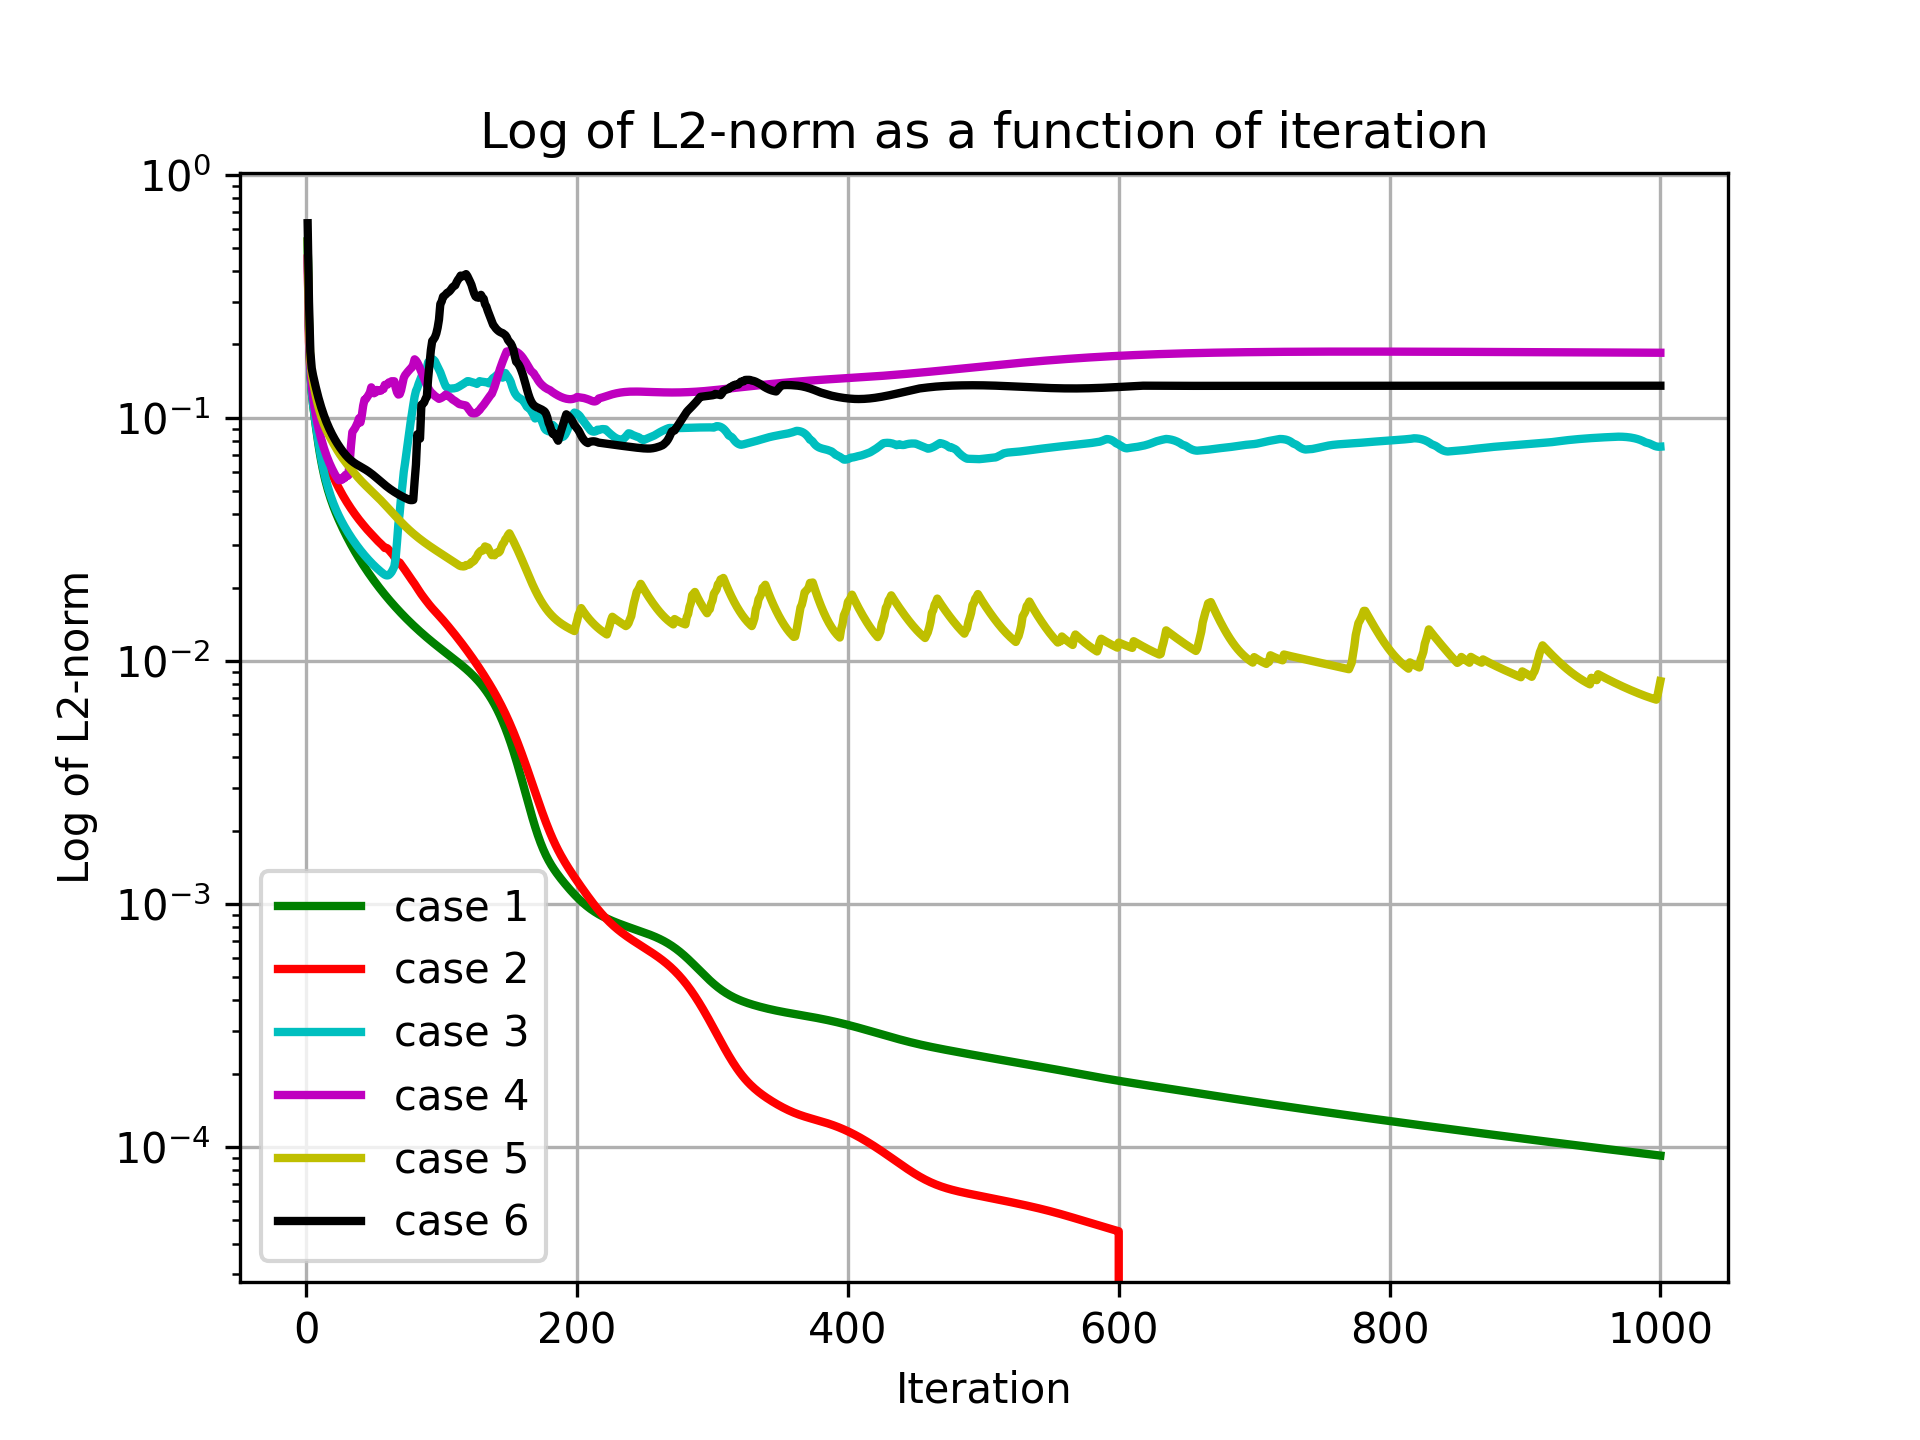
\includegraphics[width=0.75\textwidth,height=\textwidth,keepaspectratio]{images/residual_history-7.png}
    \caption{Convergence history of the six cases presented in Table \ref{tab:results}.}
    \label{fig:residual_history-7.png}
\end{figure}


\vspace{1cm}




\noindent {\bf Include a plot for the transonic cases with $M_\infty = 0.80$ showing the number of supersonic points (A$<$0) versus iteration number.}\\

Looking at case 4, we can plot the number of supersonic points per iteration number as shown in Figure \ref{fig:supersonic_points-4}. We see that the number of supersonic points begins at zero, spikes at around 30 before settling at around 25. This shows that our code is able to handle transonic cases without blowing up. 

\begin{figure}
    \centering
    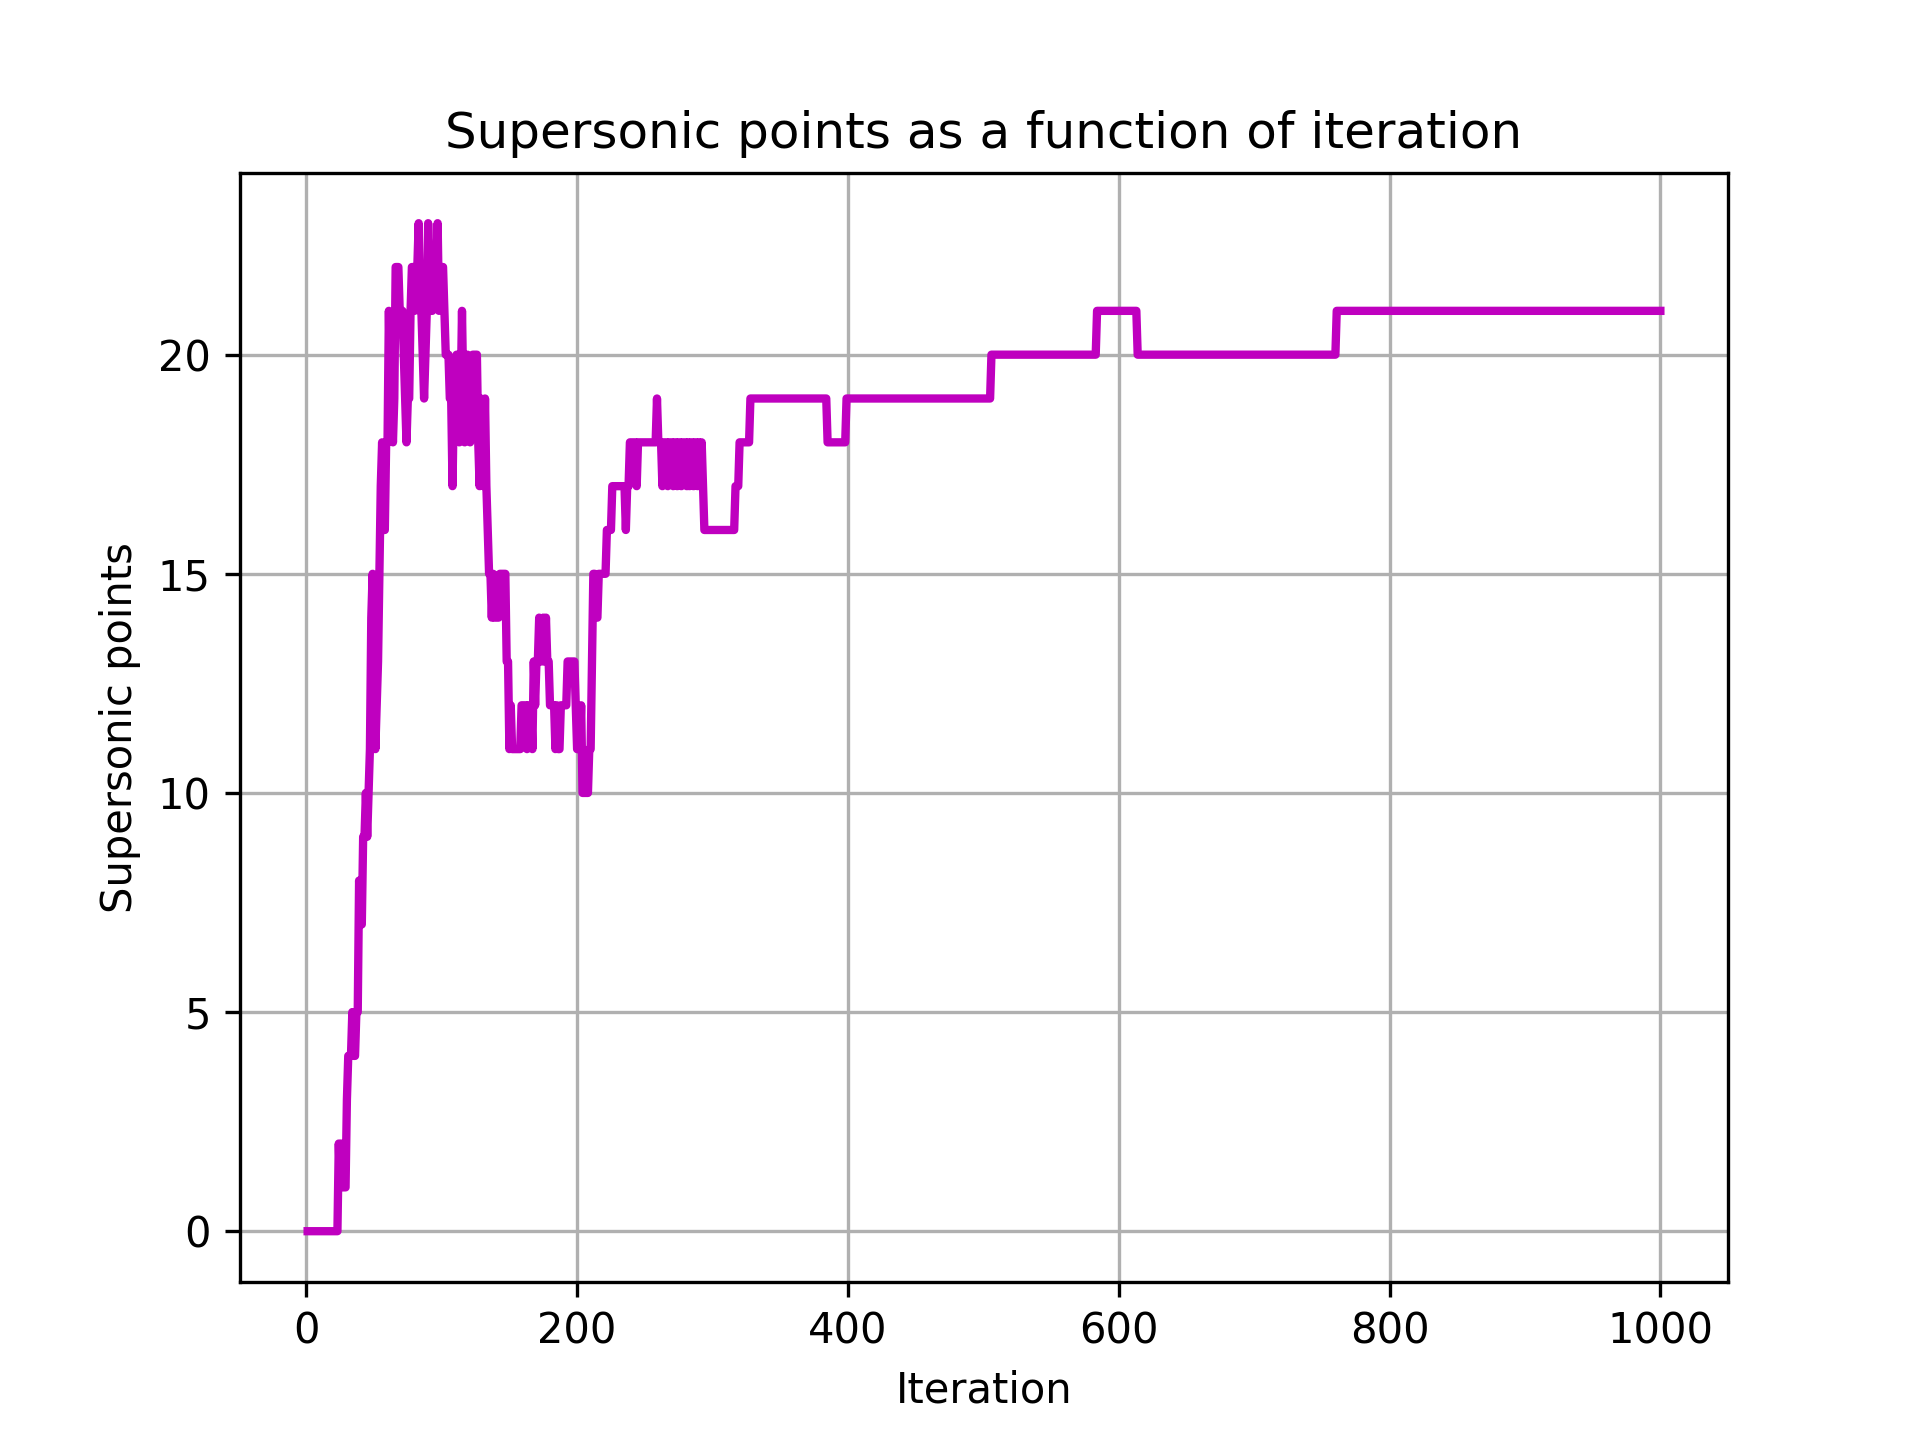
\includegraphics[width=0.75\textwidth,height=\textwidth,keepaspectratio]{images/supersonic_points-5.png}
    \caption{Number of supersonic points per iteration for a Biconvex airfoil with $M_\infty = 0.80$}
    \label{fig:supersonic_points-4}
\end{figure}

\vspace{1cm}




\noindent {\bf Note any observations and/or problems encountered. Cite any discrepancies and attempt to explain them. Are the convergence results what you expected? }\\

Looking at the convergence plots for cases 1-6 shown in Figure \ref{fig:residual_history-7.png}, we see that cases 1 and 2 show quick convergence rates while the other cases begin converging quickly but continue to flatten out after a few hundred iterations. This is a discrepancy with what we expected and is likely due to either a poor choice of relaxation parameter, we used approximately the optimal value of $1.97$, the grid not being refined enough, or a numerical error in our code. Looking at the results of case 6 where we used a stretched mesh leads us to believe that the issue may lay within our code. Furthermore, the stretched mesh should have allowed for a more accurate solution, but comparing the pressure distribution in Figure \ref{fig:pressure_coefficient-7} and Figure \ref{fig:pressure_coefficient-4}, we see that in both cases the shock was not fully resolved. Despite our best efforts, we were not able to resolve this issue in our code.

\vspace{1cm}



\noindent {\bf Plot either the velocity vector field or streamlines for one of the transonic cases, as well as contours of the potential function, pressure, and/or Mach number (you can set the limits to: $-0.5 < x < 1.5$ and $0 < y <2$).}\\

Looking at case 4, we can plot the contours of the pressure shown in Figure \ref{fig:cp_contours-5} and the velocity vector field shown in Figure \ref{fig:velocity_vectors-5}. Looking at the contour plot, we can see signs of a shock that occurred on the leading edge of the airfoil. We also note that the velocity vector field looks accurate as the flow is moving around the airfoil with signs of a boundary layer above the airfoil.

\begin{figure}
    \centering
    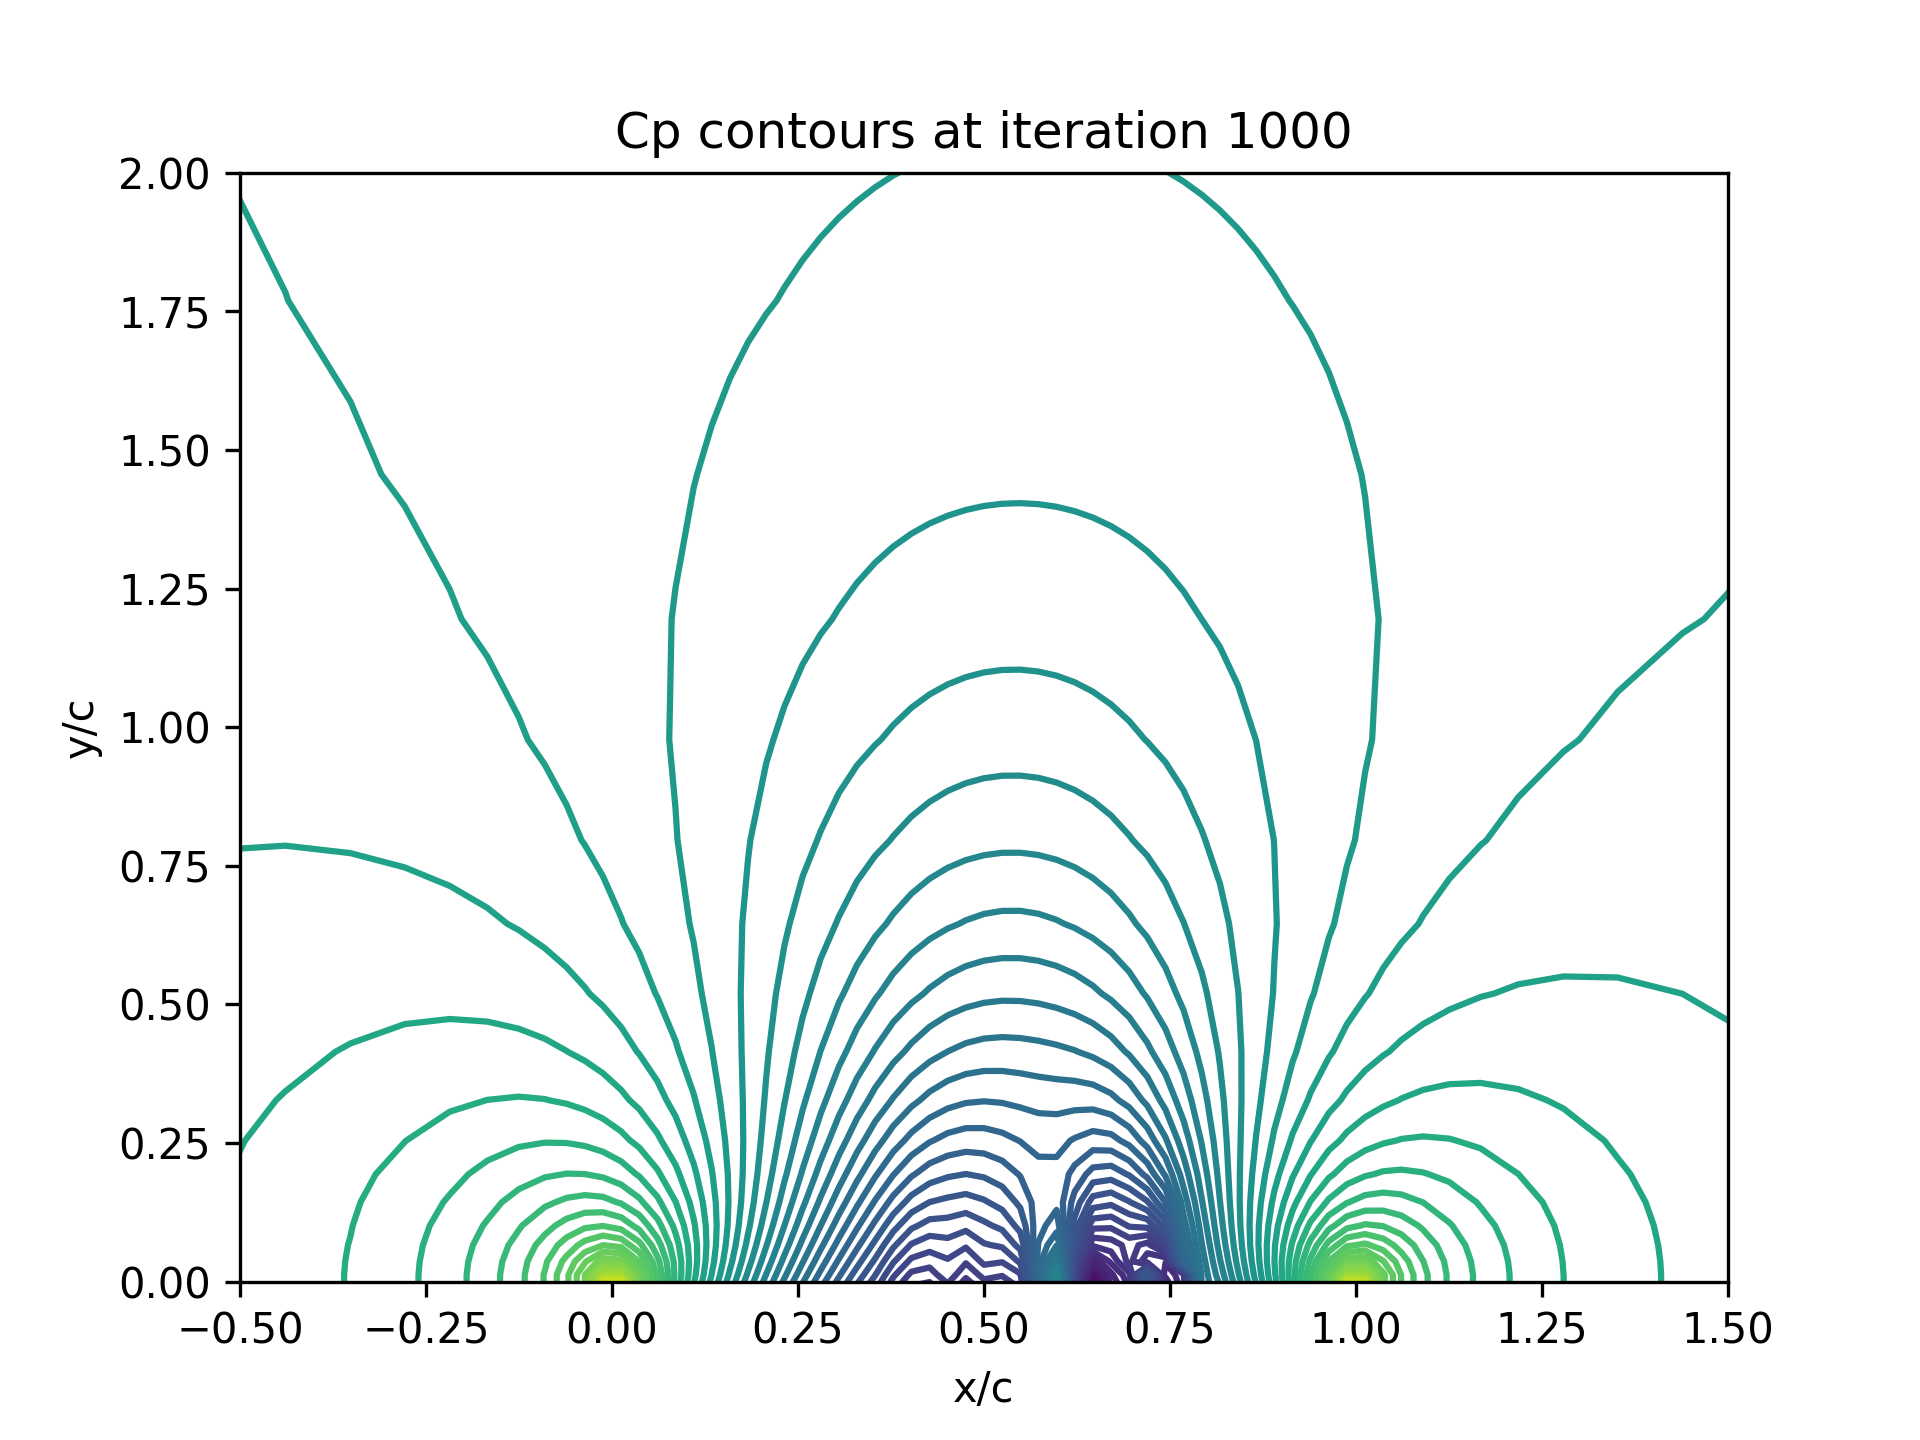
\includegraphics[width=0.75\textwidth,height=\textwidth,keepaspectratio]{images/cp_contours-5.png}
    \caption{Contour plot of $-C_p$ from $-0.5 < x < 1.5$ and $0 < y <2$ with a Biconvex airfoil with $M_\infty = 0.80$}
    \label{fig:cp_contours-5}
\end{figure}

\begin{figure}
    \centering
    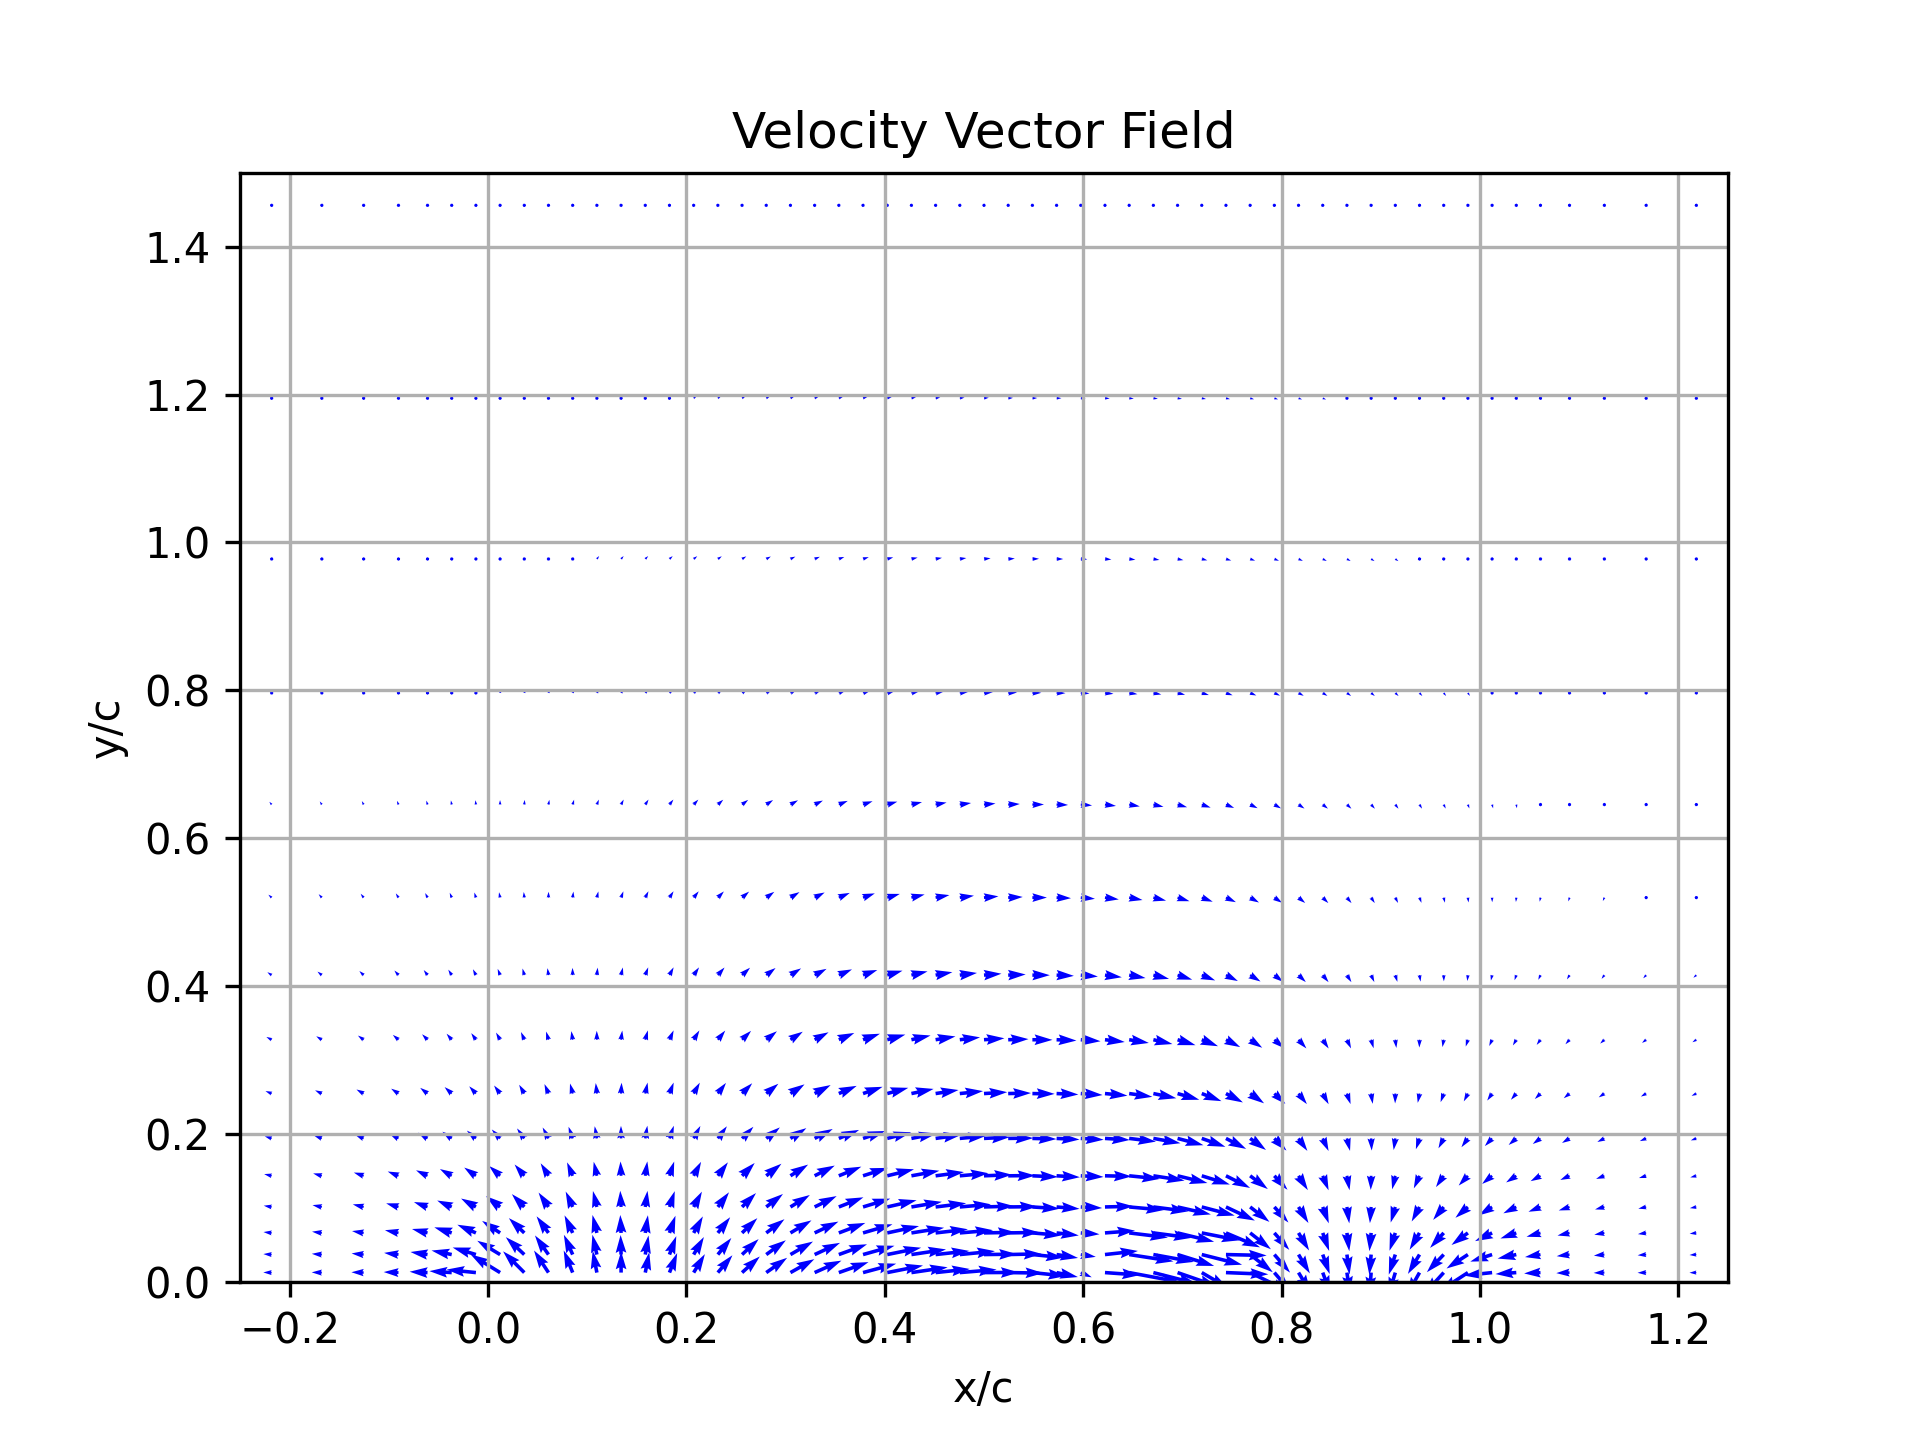
\includegraphics[width=0.75\textwidth,height=\textwidth,keepaspectratio]{images/velocity_vectors-5.png}
    \caption{Streamlines from $-0.5 < x < 1.5$ and $0 < y <2$ with a Biconvex airfoil with $M_\infty = 0.80$}
    \label{fig:velocity_vectors-5}
\end{figure}



\vspace{1cm}



\noindent {\bf Is SLOR a good method for this problem? Are the convergence characteristics what you expected? What happens if you don’t set the relaxation parameter to one in supersonic regions (explain briefly and include one plot, if helpful)? What is the effect of wind tunnel walls and/or grid parameters?}\\
Overall, SLOR is a good method for this problem. For transonic flow, if the hyperbolic regions are resolved appropriately, SLOR gives a good balance between stability and efficiency. This is shown in the convergence plot in Figure \ref{fig:residual_history-7.png}. If we don't set the relaxation number to one in supersonic regions and run case 3, we see that the code struggles to converge as show in Figure \ref{fig:res_his-4-no-omega}.

\begin{figure}
    \centering
    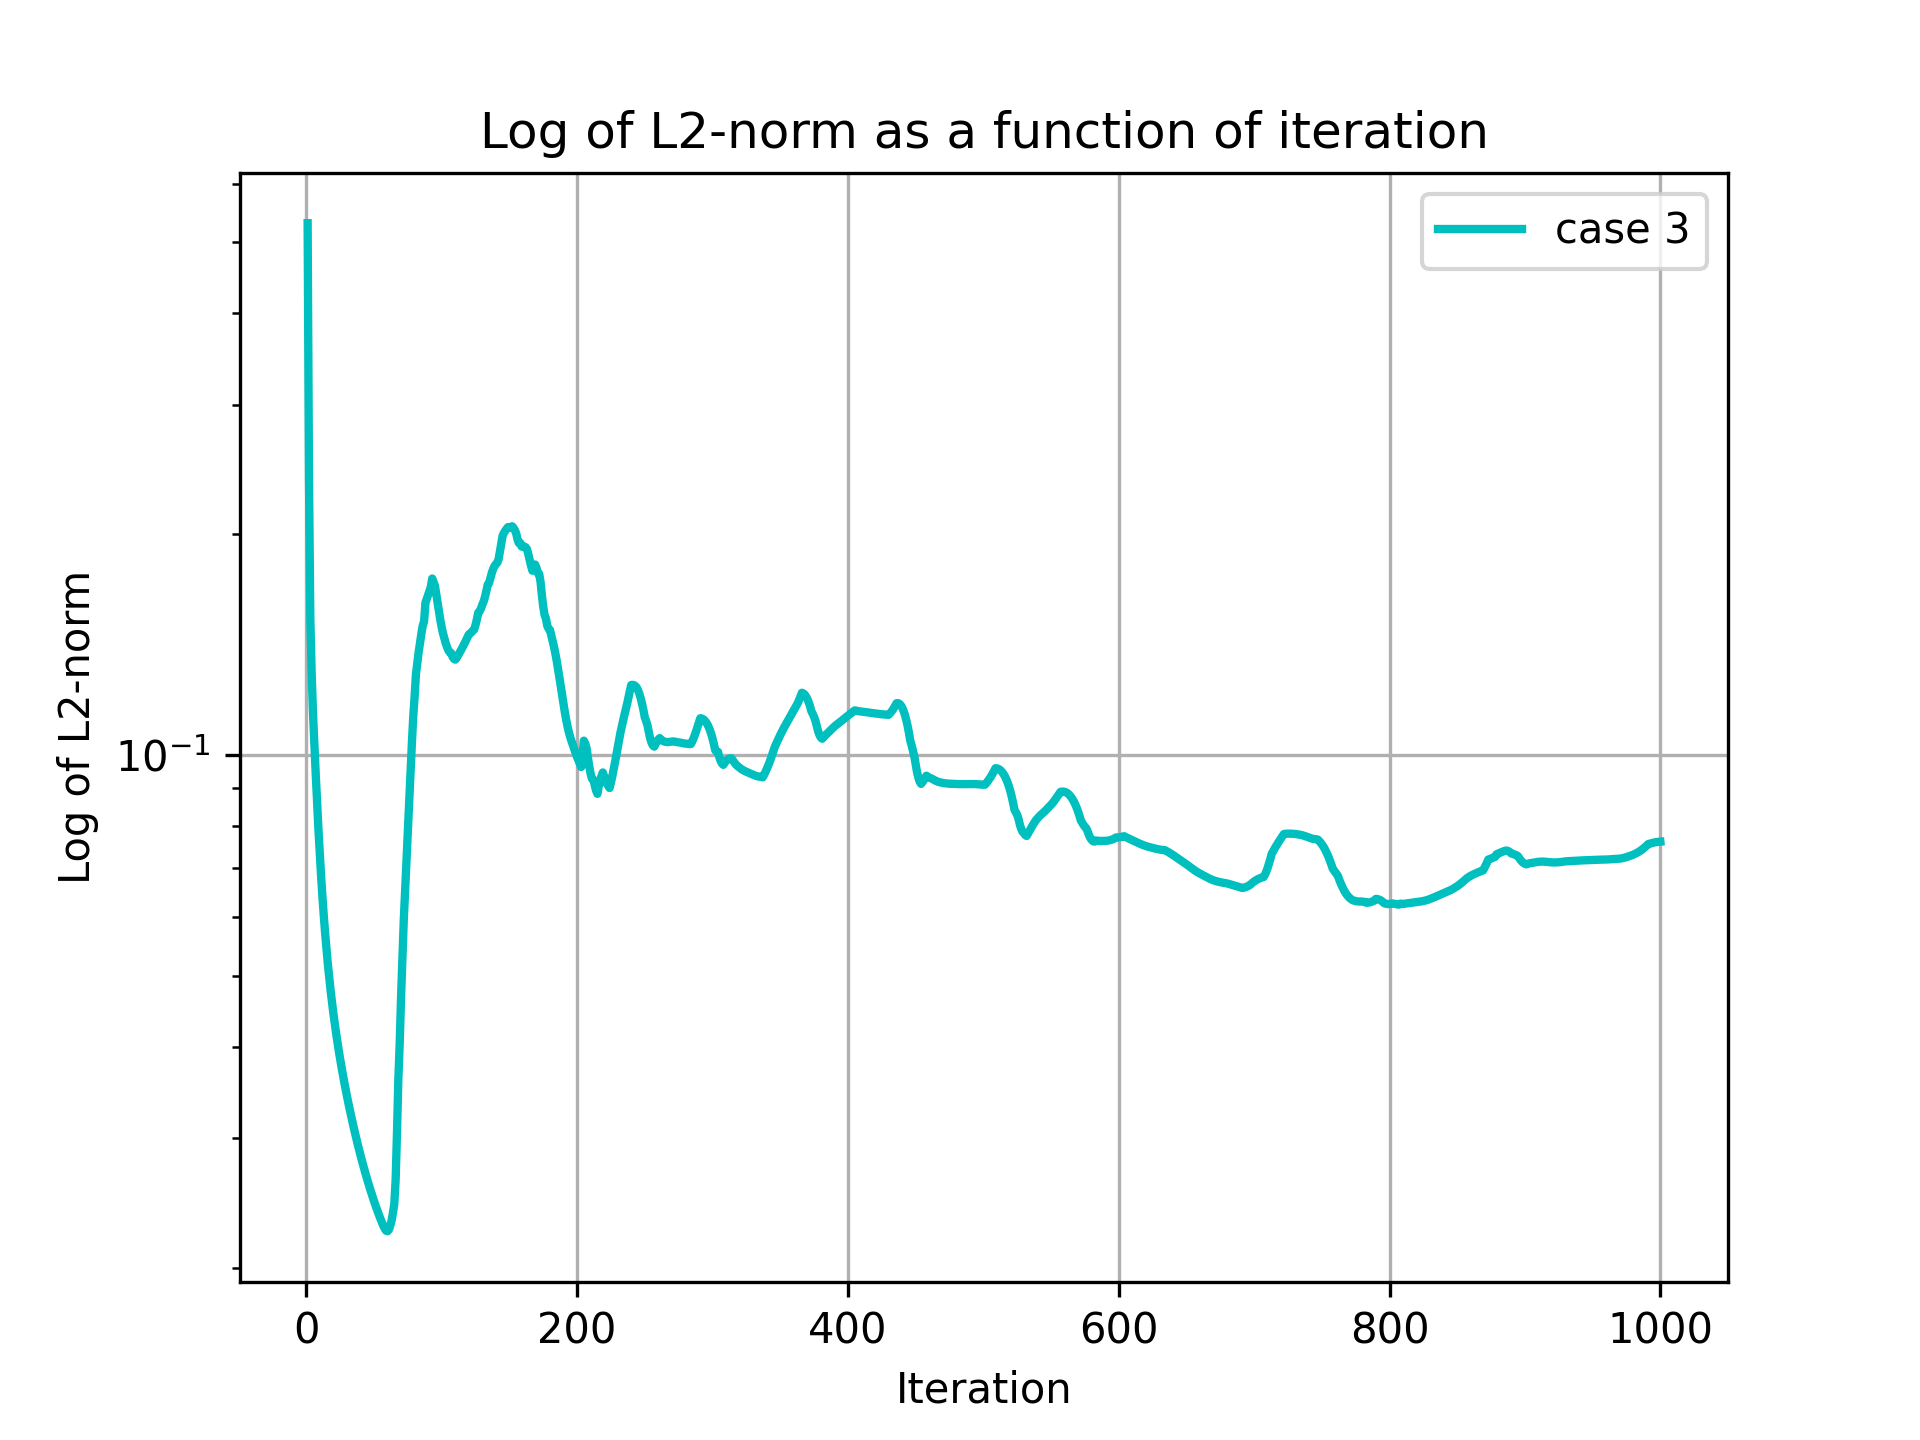
\includegraphics[width=0.75\textwidth,height=\textwidth,keepaspectratio]{images/residual_history-4-no-omega.png}
    \caption{Plot of the residual compared to the iteration count for a NACA0010 airfoil with $M_\infty = 0.80$ without adjusting $\omega = 1$ at supersonic regions.}
    \label{fig:res_his-4-no-omega}
\end{figure}


\vspace{1cm}



\noindent {\bf Briefly summarize the work, drawing conclusions and propose to your boss future modifications you could make to this code (e.g. full potential, lifting airfoil, unsteady TSD, etc.) and explain your reasoning. }\\
\\
In this work, we introduced the nonlinear small disturbance potential flow model to resolve transonic flows. This was achieved by employing different finite difference stencils in the elliptic and hyperbolic regions to align with the domain of influence. A sophisticated switch operator was implemented to efficiently transition between difference schemes. The results demonstrate that the proposed scheme effectively resolves supersonic flow, captures sonic and shock lines, and maintains computational efficiency. Additionally, pressure distributions and streamlines were analyzed to assess the solution characteristics.\\
\\
Several assumptions and simplifications were made in this study. Notably, the assumption of zero angle of attack preserves reflective symmetry along the x-axis. For future extensions, the solver can be generalized to handle lifting airfoils, which would require a more careful treatment of oblique shocks due to the increased complexity of the domain of dependence and influence.\\
\\
Currently, a three-point stencil is used in each direction, leading to second-order accuracy in the subsonic region and first-order accuracy in the supersonic region. High-resolution numerical schemes, such as WENO, could be employed to improve accuracy, particularly in handling hyperbolic problems with discontinuities.\\
\\
Although viscosity cannot be directly introduced in a potential flow model, empirical boundary layer equations could be incorporated to enhance drag and transition predictions due to viscous effects.

\vspace{1cm}



\noindent {\bf }\\

\vspace{1cm}



\noindent {\bf }\\

\vspace{1cm}



\noindent {\bf }\\

\vspace{1cm}



\noindent {\bf }\\

\vspace{1cm}


\newpage
\noindent \textbf{Appendix: code of this project}\\
\tiny
\begin{verbatim}
import numpy as np
import matplotlib.pyplot as plt
from math import sqrt
import time

from tri import solve_tridiagonal

colors = ['b', 'g', 'r', 'c', 'm', 'y', 'k']

def main(condition=0, show_plots=True, show_prints=True):
    # -------------------------------------------------------------------------
    # Parameters 
    # -------------------------------------------------------------------------
    thickness = 0.10                         # Airfoil thickness

    # SLOR parameters
    omega = 1.97
    itmax = 1000
    itplot = 200
    
    gamma = 1.4

    # Mesh input parameters
    
    # case from hw3
    if condition == 1:
        j_le = 33     # leading edge index
        j_te = 63     # trailing edge index
        jmax = 95     # total x points
        kmax = 33     # total y points
        xsf = 1.18    # x stretching factor
        ysf = 1.18    # y stretching factor
        airfoil_type = 0   # airfoil type - 0 for NACA0010 and 1 for biconvex airfoil
        minf = 0.0
    elif condition == 7:
        j_le = 63
        j_te = 123
        jmax = 185
        kmax = 63
        xsf = 1.1
        ysf = 1.0
        airfoil_type = 0   # airfoil type - 0 for NACA0010 and 1 for biconvex airfoil
        minf = 0.8
    else:
        j_le = 33
        j_te = 73
        jmax = 105
        kmax = 43
        xsf = 1.2
        ysf = 1.2
        if condition == 2:
            minf = .75
            airfoil_type = 0
        elif condition == 3:
            minf = 0.75
            airfoil_type = 1
        elif condition == 4:
            minf = 0.8
            airfoil_type = 0
        elif condition == 5:
            minf = 0.8
            airfoil_type = 1
        elif condition == 6:
            minf = 0.75
            airfoil_type = 0
            ysf = 1.0


    
    kconst = 3      # number of constant-spaced mesh points
    dxdy = 1.0      # ratio of dx to dy at airfoil surface

    # Upper wall boundary?
    if condition == 6:
        iwall = 1
    else:
        iwall = 0
    if iwall == 1:
        ysf = 1.0
    ibc = 0         # Use full bc if 0, or simplified if 1

    # -------------------------------------------------------------------------
    # Mesh Generation
    # -------------------------------------------------------------------------
    # Generate x-array
    dx1 = 1.0 / (j_te - j_le + 1)      # equal spacing along airfoil
    dy1 = dx1 / dxdy
    # Create x coordinates 
    x = np.zeros(jmax)
    for j in range(jmax):
        # MATLAB: x(j) = (j - j_le)*dx1 + 0.5*dx1, j=1...jmax => Python index: j = 0...jmax-1, j+1 used
        x[j] = ((j + 1) - j_le) * dx1 + 0.5 * dx1

    # Upstream stretching
    # Convert: for i from (j_le - kconst - 1) down to 1 (MATLAB) => Python indices: from (j_le - kconst - 1 - 1) down to 0.
    for i in range(j_le - kconst - 2, -1, -1):
        x[i] = x[i+1] + (x[i+1] - x[i+2]) * xsf


    # Downstream stretching 
    for i in range(j_te + kconst, jmax):
        x[i] = x[i-1] + (x[i-1] - x[i-2]) * xsf

    # Generate y-array
    y = np.zeros(kmax)
    for k in range(kmax):
        # y(k) = (k-1)*dy1 - 0.5*dy1, k=1...kmax
        y[k] = (k) * dy1 - 0.5 * dy1

    # Stretching in y-direction for interior points (MATLAB: for ki=kconst+1:kmax-kconst)
    for k in range(kconst, kmax - kconst):
        y[k] = y[k-1] + (y[k-1] - y[k-2]) * ysf
    # Outermost points: uniform spacing
    for k in range(kmax - kconst, kmax):
        y[k] = y[k-1] + (y[k-1] - y[k-2])

    # Create 2D mesh arrays
    xmesh = np.zeros((jmax, kmax))
    ymesh = np.zeros((jmax, kmax))
    for k in range(kmax):
        for j in range(jmax):
            xmesh[j, k] = x[j]
            ymesh[j, k] = y[k]

    # Calculate spacing in x-direction
    dx = np.full(jmax, dx1)
    for j in range(1, jmax-1):
        dx[j] = 0.5 * (x[j+1] - x[j-1])
    dx[0] = 2 * dx[1] - dx[2]
    dx[-1] = 2 * dx[-2] - dx[-3]

    # Calculate arrays for mesh scaling in x-direction
    dxp2 = 1.0 / (dx ** 2)
    dxm2 = 1.0 / (dx ** 2)
    for j in range(1, jmax-1):
        dxp2[j] = 1 / (dx[j]* (x[j+1] - x[j]))
        dxm2[j] = 1 / (dx[j]* (x[j] - x[j-1]))
        
    # set initial things
    dxp2[0] = dxp2[1]
    dxm2[0] = dxm2[1]

    # Calculate spacing in y-direction
    dy = np.full(kmax, dy1)
    dy[0] = y[1] - y[0]
    for k in range(1, kmax-1):
        dy[k] = 0.5 * (y[k+1] - y[k-1])
    dy[-1] = 2 * dy[-2] - dy[-3]

    # Calculate arrays for mesh scaling in y-direction
    dyp2 = 1.0 / (dy ** 2)
    dym2 = 1.0 / (dy ** 2)
    for k in range(1, kmax-1):
        dyp2[k] = 1 / (dy[k] * (y[k+1] - y[k]))
        dym2[k] = 1 / (dy[k] * (y[k] - y[k-1]))

    # -------------------------------------------------------------------------
    # Initialization
    # -------------------------------------------------------------------------
    phi = np.zeros((jmax, kmax))
    # Incompressible potential data for NACA0010 (Abbott and von Doenhoff)
    potx = np.array([0.0, 0.005, 0.0125, 0.025, 0.050, 0.075, 0.1, 0.15, 0.2, 0.25,
                     0.3, 0.4, 0.5, 0.6, 0.7, 0.8, 0.9, 0.95, 1.0])
    potcp = np.array([1.0, 0.282, -0.061, -0.237, -0.325, -0.341, -0.341, -0.341,
                      -0.329, -0.309, -0.284, -0.237, -0.190, -0.138, -0.094, -0.040,
                      0.04, 0.075, 1.0]) 
    if show_prints:
        print("DX1 is", dx1, "DY1 is", dy1)
        print("XMAX is", x[-1], "YMAX is", y[-1])
    
    # Plot the initial mesh
    fig1 = plt.figure()
    ax1 = fig1.add_subplot(111, projection='3d')
    ax1.plot_wireframe(xmesh, ymesh, phi, rstride=2, cstride=2)
    ax1.set_title('Mesh')
    ax1.set_xlabel('x/c')
    ax1.set_ylabel('y/c')
    

    # Pre-allocate arrays for SLOR iterations
    a = np.zeros(kmax)
    b = np.zeros(kmax)
    c = np.zeros(kmax)
    f_arr = np.zeros(kmax)
    cpg = np.zeros((jmax, kmax))
    cp = np.zeros(jmax)
    cpu = np.zeros(jmax)
    res = np.zeros((jmax, kmax))
    l2reshist = np.zeros(itmax)
    
    istop = False
    l2res1 = None
    supersonic_points = np.zeros(itmax) 
    # -------------------------------------------------------------------------
    # SLOR Iterations
    # -------------------------------------------------------------------------
    for it in range(1, itmax+1):
        if istop:
            break

        # --- Apply boundary condition along airfoil (k=0 corresponds to k=1 in MATLAB) ---
        bc = np.zeros(jmax)
        # Loop from j_le to j_te (MATLAB indices) => Python indices: j_le-1 to j_te-1
        for j in range(j_le - 1, j_te):
            # NACA00xx airfoil
            if airfoil_type == 0:
                x_int = 1.008930411365  # NACA00xx airfoil slope constant
                # Avoid division by zero in sqrt; x[j] is positive in the airfoil region
                dphidy = 5 * thickness * (0.2969 * 0.5 * sqrt(x_int / x[j])
                                        - 0.126 * x_int
                                        - 0.3516 * 2 * x_int**2 * x[j]
                                        + 0.2843 * 3 * x_int**3 * x[j]**2
                                        - 0.1015 * 4 * x_int**4 * x[j]**3)
            # Biconvex airfoil
            elif airfoil_type == 1:
                dphidy = 2 * thickness * (1 - 2 * x[j])

            # Compute velocity in x-direction using central differences
            velx = 0.5 * (
                ((phi[j+1, 0] - phi[j, 0]) / dx[j]) * (dxp2[j] / dxm2[j]) +
                ((phi[j, 0] - phi[j-1, 0]) / dx[j]) * (dxm2[j] / dxp2[j])
            )
            if ibc == 1:
                velx = 0.0  # simplified boundary condition
            bc[j] = -dphidy * (1.0 + velx) * dy[0]

        # Apply airfoil boundary condition (k=0)
        for j in range(jmax):
            phi[j, 0] = phi[j, 1] + bc[j]

        # Upper wall boundary condition if applicable (kmax-1 corresponds to kmax in MATLAB)
        if iwall == 1:
            for j in range(jmax):
                phi[j, kmax-1] = phi[j, kmax-2]

        # Compute A matrix
        A = np.zeros((jmax, kmax))
        for j in range(1, jmax-1):
            for k in range(1, kmax-1):
                A[j, k] = 1 - minf**2 - minf**2*(gamma + 1) * 1 * 1/(x[j+1] - x[j-1]) * ( (phi[j+1, k] - phi[j, k]) * (x[j] - x[j-1]) / (x[j+1] - x[j]) \
                    + (phi[j, k] - phi[j-1, k]) * (x[j+1] - x[j]) / (x[j] - x[j-1]))

                
        # --- Calculate residual and its L2 norm ---
        l2res = 0.0
        for k in range(1, kmax-1):
            for j in range(1, jmax-1):
                res[j, k] = (A[j,k] *
                             ((phi[j+1, k] - phi[j, k]) * dxp2[j] - (phi[j, k] - phi[j-1, k]) * dxm2[j])
                             + ((phi[j, k+1] - phi[j, k]) * dyp2[k] - (phi[j, k] - phi[j, k-1]) * dym2[k]))
                
                l2res += res[j, k] ** 2
        l2res = sqrt(l2res / (jmax * kmax))
        if it == 1:
            l2res1 = l2res
        
        # Stop condition if residual changes too much
        if l2res1 / l2res >= 10000 or l2res1 / l2res <= 1.0 / 1000:
            istop = True
        
        if show_prints:
            print(f"Iteration {it} : L2(RES) = {l2res}")
        
        mu = np.where(A >= 0, 0, 1)
        omega_jk = np.ones((jmax, kmax)) * omega
        omega_jk[A < 0] = 1
        
        
        # --- SLOR update using tridiagonal solver along each interior x-row ---
        dphi = np.zeros((jmax, kmax))
        for j in range(1, jmax-1):
            # Set up the tridiagonal system for row j
            # k = 0 (airfoil boundary)
            a[0] = 0.0
            b[0] = 1.0
            c[0] = -1.0
            f_arr[0] = 0.0
            # Interior points k = 1 to kmax-2
            for k in range(1, kmax-1):
                a[k] = dym2[k]
                b[k] = -(1  - mu[j,k]) *(dym2[k] + dyp2[k] + A[j,k] * (dxm2[j] + dxp2[j])) + mu[j-1,k] * A[j-1,k] * dxp2[j-1]
                c[k] = dyp2[k]
                f_arr[k] = -omega_jk[j,k] * (1  - mu[j,k]) *  A[j,k] * (res[j, k] + dphi[j-1, k] * dxm2[j]) - mu[j-1,k] * omega_jk[j,k] * A[j-1,k] * ((dxp2[j-1] + dxm2[j-1]) * dphi[j-1, k] - dxm2[j-1] * dphi[j-2, k])
            # k = kmax-1 (upper boundary)
            a[kmax-1] = 0.0
            b[kmax-1] = 1.0
            c[kmax-1] = 0.0
            f_arr[kmax-1] = 0.0
            if iwall == 1:
                a[kmax-1] = -1.0
            # Solve tridiagonal system for this row
            dphi[j, :] = solve_tridiagonal(a.copy(), b.copy(), c.copy(), f_arr.copy())
        
        # Update solution
        phi = phi + dphi
        l2reshist[it-1] = l2res

        # --- Calculate pressure coefficients along the airfoil and upper boundary ---
        cp[0] = -2 * ((phi[1, 0] - phi[0, 0]) / (x[1] - x[0]))
        cpu[0] = -2 * ((phi[1, kmax-1] - phi[0, kmax-1]) / (x[1] - x[0]))
        for j in range(1, jmax-1):
            cp[j] = -2 * 0.5 * (
                ((phi[j+1, 0] - phi[j, 0]) / dx[j]) * (dxp2[j] / dxm2[j]) +
                ((phi[j, 0] - phi[j-1, 0]) / dx[j]) * (dxm2[j] / dxp2[j])
            )
            cpu[j] = -2 * 0.5 * (
                ((phi[j+1, kmax-1] - phi[j, kmax-1]) / dx[j]) * (dxp2[j] / dxm2[j]) +
                ((phi[j, kmax-1] - phi[j-1, kmax-1]) / dx[j]) * (dxm2[j] / dxp2[j])
            )
        cp[-1] = -2 * ((phi[-1, 0] - phi[-2, 0]) / (x[-1] - x[-2]))
        cpu[-1] = -2 * ((phi[-1, kmax-1] - phi[-2, kmax-1]) / (x[-1] - x[-2]))
        
        # --- Compute number of supersonic points ---
        supersonic_point = np.sum(A < 0)
        # supersonic_points.append(supersonic_point)
        supersonic_points[it-1] = supersonic_point
        
        if show_prints:
            print(f"Number of supersonic points: {supersonic_points}")

        
        # Plot Cp contours if required
        if it < 10 or it % itplot == 0:
            for k in range(kmax):
                # k=0 boundary
                cpg[0, k] = -2 * ((phi[1, k] - phi[0, k]) / (x[1] - x[0]))
                for j in range(1, jmax-1):
                    cpg[j, k] = -2 * 0.5 * (
                        ((phi[j+1, k] - phi[j, k]) / dx[j]) * (dxp2[j] / dxm2[j]) +
                        ((phi[j, k] - phi[j-1, k]) / dx[j]) * (dxm2[j] / dxp2[j])
                    )
                cpg[-1, k] = -2 * ((phi[-1, k] - phi[-2, k]) / (x[-1] - x[-2]))
            if show_plots:
                plt.figure(2)
                plt.clf()
                cp_levels = 50
                cp_contours = plt.contour(xmesh, ymesh, cpg, cp_levels)
                plt.axis([-0.25, 1.25, 0.0, 1.5])
                plt.title(f'Cp contours at iteration {it}')
                plt.xlabel('x/c')
                plt.ylabel('y/c')
                # plt.pause(0.001)
    
    # Plot pressure coefficient along airfoil and upper wall
    if show_plots:
        plt.figure(3)
        plt.clf()
        plt.plot(x, -cp, 'm', marker='o', linewidth=2, markersize=10, label='Airfoil')
        plt.plot(x, -cpu, 'r', marker='+', linewidth=2, markersize=10, label='Upper wall')
        plt.plot(potx, -potcp/np.sqrt(1 - minf**2), 'gx', linewidth=2, markersize=10, label='External Data')
        plt.axis([-0.25, 1.25, -1.4, 1.0])
        plt.title(f'-Cp as a function of x/c at iteration {it}')
        plt.xlabel('x/c')
        plt.ylabel('-Cp')
        plt.grid(True)
        plt.legend()
        plt.savefig(f"images/pressure_coefficient-{condition}.png", dpi=300)
        # plt.pause(0.001)
    
    # Plot the residual history
    if show_plots:
        plt.figure(4)
        # plt.clf()
        plt.semilogy(range(1, it+1), l2reshist[:it], 'm-', color=colors[condition-1], linewidth=2, label=f'case {condition-1}')
        plt.title('Log of L2-norm as a function of iteration')
        plt.xlabel('Iteration')
        plt.ylabel('Log of L2-norm')
        plt.legend()
        

        plt.grid(True)
        plt.figure(4)
        plt.savefig(f"images/residual_history-{condition}.png", dpi=300)
                    
    # plot supersonic points per iteration
    if show_plots:
        plt.figure(6)
        plt.clf()
        plt.plot(range(1, it+1), supersonic_points[:it], 'm-', linewidth=2)
        plt.title('Supersonic points as a function of iteration')
        plt.xlabel('Iteration')
        plt.ylabel('Supersonic points')
        plt.grid(True)
        plt.savefig(f"images/supersonic_points-{condition}.png", dpi=300)
    
    # plot the final Cp contours
    if show_plots:
                plt.figure(2)
                plt.clf()
                cp_levels = 50
                cp_contours = plt.contour(xmesh, ymesh, cpg, cp_levels)
                plt.axis([-0.5, 1.5, 0.0, 2])
                plt.title(f'Cp contours at iteration {it}')
                plt.xlabel('x/c')
                plt.ylabel('y/c')
                plt.savefig(f"images/cp_contours-{condition}.png", dpi=300)
  
    # Plot streamlines
    if show_plots:
            # Compute velocity components from potential phi
        u = np.zeros((jmax, kmax))
        v = np.zeros((jmax, kmax))

        # Compute derivatives using central differences
        for j in range(1, jmax - 1):
            for k in range(1, kmax - 1):
                u[j, k] = (phi[j+1, k] - phi[j-1, k]) / (x[j+1] - x[j-1])
                v[j, k] = (phi[j, k+1] - phi[j, k-1]) / (y[k+1] - y[k-1])
                
        plt.figure()
        plt.quiver(xmesh, ymesh, u, v, color='b', scale=10)
        plt.title('Velocity Vector Field')
        plt.xlabel('x/c')
        plt.ylabel('y/c')
        plt.axis([-0.25, 1.25, 0.0, 1.5])
        plt.grid(True)
        plt.savefig(f"images/velocity_vectors-{condition}.png", dpi=300)
    
    return supersonic_point, minf, airfoil_type, it

\end{verbatim}

\large
\noindent \textbf{Appendix: Sample output of code}\\
\tiny
\begin{verbatim}
====================================
Running condition 1
Airfoil: NACA0010 with M_inf = 0.75, and 0 supersonic points found in 1000 iterations
Elapsed time: 19.90214776992798 seconds
====================================
====================================
Running condition 2
Airfoil: Biconvex with M_inf = 0.75, and 0 supersonic points found in 601 iterations
Elapsed time: 12.052074432373047 seconds
====================================
====================================
Running condition 3
Airfoil: NACA0010 with M_inf = 0.8, and 10 supersonic points found in 1000 iterations
Elapsed time: 20.13447380065918 seconds
====================================
====================================
Running condition 4
Airfoil: Biconvex with M_inf = 0.8, and 21 supersonic points found in 1000 iterations
Elapsed time: 19.85328221321106 seconds
====================================
====================================
Running condition 5
Airfoil: NACA0010 with M_inf = 0.75, and 1 supersonic points found in 1000 iterations
Elapsed time: 20.19430923461914 seconds
====================================
====================================
Running condition 6
Airfoil: NACA0010 with M_inf = 0.8, and 18 supersonic points found in 1000 iterations
Elapsed time: 52.96372580528259 seconds
====================================
\end{verbatim}

\large
\noindent \textbf{Appendix: Sample input of code}\\
\tiny
\begin{verbatim}
def collect_times():
    for i in range(2, 8):
        print("====================================")
        print(f"Running condition {i}")
        start_time = time.time()
        supersonic_points, minf, airfoil_type, final_iteration = main(i, False, False)
        end_time = time.time()
        airfoil_name = "NACA0010" if airfoil_type == 0 else "Biconvex"
        print(f"Airfoil: {airfoil_name} with M_inf = {minf}, and {supersonic_points} supersonic points found in {final_iteration} iterations")
        print("Elapsed time:", end_time - start_time, "seconds")
        print("====================================")

def collect_figures():
    for i in range(5, 6):
        print(f"Running condition {i}")
        supersonic_points, minf, airfoil_type, final_iteration = main(i, True, False)

if __name__ == '__main__':
    collect_times()
    collect_figures()    
\end{verbatim}


\end{document}
